\section{Grundlegende Begriffe}

Zur Erinnerung werden wir in diesem Abschnitt einige grundlegende Begriffe aus der Maßtheorie und der Stochastik wiederholen. Die meisten Definitionen und Sätze lassen sich in ähnlicher Form auch in \cite{Klenke} und \cite{Meintrup} finden. Da dies Grundlagen aus Maß- und Wahrscheinlichkeitstheorie sind, wurde auf entsprechende Zitate verzichtet.

\subsection{Zufallsvariablen}

Die Objekte, mit denen wir uns im Folgenden beschäftigen wollen, sind reelle Zufallsvariablen. Dazu benötigen wir zunächst folgende

\begin{Definition}{($\sigma$-Algebra)}
\hypertarget{Def:Sigma}{}Sei $\Omega$ eine beliebige Menge und $\mathscr{A} \subseteq \mathcal{P}(\Omega)$ ein Mengensystem. Gilt
\begin{enumerate}[label=\textup{(S\arabic*)}]
\item $\Omega \in \mathscr{A}$
\item $\forall A \in \mathscr{A}: A^\complement \in \mathscr{A}$
\item $\forall (A_n)_{n \in \mathbb{N}_0} \subseteq \mathscr{A}: \bigcup_{n \in \mathbb{N}_0} A_n \in \mathscr{A}$~,
\end{enumerate}
so ist $\mathscr{A}$ eine \textit{$\sigma$-Algebra} und $(\Omega, \mathscr{A})$ ein \textit{Messraum}.
\end{Definition}

Die Eigenschaft (S2) bezeichnet man auch als \textit{Komplementstabilität} und die Eigenschaft (S3) als \textit{$\sigma$-Vereinigungsstabilität}.

\begin{Beispiel}{($\sigma$-Algebren)}
Wir werden nun einige einfache und häufig vorkommende Beispiele für $\sigma$-Algebren betrachten. Gegeben sei zunächst eine beliebige Menge $\Omega$.
\begin{enumerate}[label=(\roman*)]
\item Die kleinste (\textit{gröbste}) $\sigma$-Algebra ist gegeben durch
\[\mathscr{A} = \{ \emptyset, \Omega \}~.\]
\item Die größte (\textit{feinste}) $\sigma$-Algebra ist gegeben durch
\[\mathscr{A} = \mathcal{P}(\Omega)~.\]
Ist $\Omega$ höchstens abzählbar, so verwenden wir genau diese Potenzmenge als $\sigma$-Algebra.
\end{enumerate}
Sei nun $\Omega = \mathbb{R}$ die reellen Zahlen.
\begin{enumerate}[label=(\roman*), resume]
\item In diesem Fall verwenden wir die \textit{Borelsche-$\sigma$-Algebra}
\[\mathscr{A} = \mathscr{B}~.\]
Diese wird erzeugt von den offenen Mengen.
\end{enumerate}
Sei weiter $\Omega = [a, b]$ ein reelles Intervall mit $a < b$.
\begin{enumerate}[label=(\roman*), resume]
\item In diesem Fall verwenden wir auch die \textit{Borelsche-$\sigma$-Algebra}, müssen sie aber folgendermaßen einschränken
\begin{align*}
\mathscr{A} &= \mathscr{B}_{[a, b]}\\
&= \{ B \cap [a, b] \mid B \in \mathscr{B} \}~.
\end{align*}
Diese Konstruktion verläuft auch analog für andere Borel-Mengen.
\end{enumerate}
\end{Beispiel}

\newpage

Mit diesen Begriffen können wir nun Messbarkeit definieren.

\begin{Definition}{(Messbarkeit)}
Gegeben seien zwei Messräume $(\Omega_1, \mathscr{A}_1)$ und $(\Omega_2, \mathscr{A}_2)$, sowie eine Abbildung $f: (\Omega_1, \mathscr{A}_1) \rightarrow (\Omega_2, \mathscr{A}_2)$. Gilt für alle $A_2 \in \mathscr{A}_2$
\[f^{-1}(A_2) \in \mathscr{A}_1~,\]
so nennt man $f$ \textit{$\mathscr{A}_1$-$\mathscr{A}_2$-messbar} oder kurz \textit{messbar}.
\end{Definition}

Wir wollen nun ein paar Beispiele für messbare Abbildungen betrachten.

\begin{Beispiel}{(Messbare Abbildungen)}
\begin{enumerate}[label=(\roman*)]
\item Gegeben sei $(\mathbb{R}, \mathscr{B})$ und $f \in \mathcal{C}^0(\mathbb{R}, \mathbb{R})$ eine stetige Funktion. Dann ist $f$ messbar. Sei $O_2 \in \mathscr{B}$ eine offene Menge. Nach Definition der Stetigkeit existiert eine weitere offene Menge $O_1 \in \mathscr{B}$, sodass
\[f^{-1}(O_2) = O_1\]
ist. Da die Borelschen-$\sigma$-Algebra von den offenen Mengen erzeugt wird, ist $f$ messbar.

\item Gegeben sei $(\Omega, \mathscr{A})$ und ein $A \in \mathscr{A}$. Dann ist $\indi_A$ messbar. Sei $B \in \mathscr{B}$. Betrachte nun die folgenden Fallunterscheidung

{
\renewcommand{\arraystretch}{1.5}
\begin{tabularx}{0.5\linewidth}{X X}
$0, 1 \in B$ & $\indi_B^{-1}(B) = \mathbb{R}$\\
$0 \in B, 1 \notin B$ & $\indi_B^{-1}(B) = A^\complement$\\
$0 \notin B, 1 \in B$ & $\indi_B^{-1}(B) = A$\\
$0, 1 \notin B$ & $\indi_B^{-1}(B) = \emptyset$
\end{tabularx}
}

Alle Mengen rechts sind nach \hyperlink{Def:Sigma}{\blue{Definition}} in der Borel-$\sigma$-Algebra.

\item Gegeben sei $\Omega = \{\omega_1, \omega_2, \omega_3\}$ und $\mathscr{A} = \{ \emptyset, \{\omega_1, \omega_2\}, \{\omega_3\}, \Omega\}$. Weiter sei
\begin{align*}
f: (\Omega, \mathscr{A}) \rightarrow (\{0, 1\}, \mathcal{P}(\{0, 1\})):~ &\omega_1 \mapsto 0\\
&\omega_2 \mapsto 0\\
&\omega_3 \mapsto 1~.
\end{align*}
Es gilt
\[\mathcal{P}(\{0, 1\}) = \{ \emptyset, \{0\}, \{1\}, \{0, 1\} \}~.\]
Betrachte also
\begin{align*}
f^{-1}(\emptyset) &= \emptyset\\
f^{-1}(\{0\}) &= \{\omega_1, \omega_2\}\\
f^{-1}(\{1\}) &= \{\omega_3\}\\
f^{-1}(\{0, 1\}) &= \Omega~.
\end{align*}
Da all diese Mengen in $\mathscr{A}$ liegen, ist $f$ messbar. Verwenden wir hingegen $\{\emptyset, \Omega\}$ als $\sigma$-Algebra, so ist $f$ nicht mehr messbar, da das Urbild von $\{0\}$ nicht in der $\sigma$-Algebra liegt.
\end{enumerate}
Vor allem an diesem letzten Beispiel sehen wir, dass Messbarkeit stark von den verwendeten $\sigma$-Algebren abhängt.
\end{Beispiel}

\newpage

Um unsere Reise durch die Maßtheorie fortsetzen zu können, benötigen wir noch das namensgebende Maß.

\begin{Definition}{(Maß)}
\hypertarget{Def:Maß}{}Sei $(\Omega, \mathscr{A})$ ein Messraum und $\mu: \mathscr{A} \rightarrow \overline{\mathbb{R}}$ eine Abbildung. Gilt
\begin{enumerate}[label=\textup{(M\arabic*)}]
\item $\mu(\emptyset) = 0$
\item $\forall A \in \mathscr{A}: \mu(A) \geq 0$
\item $\forall (A_n)_{n \in \mathbb{N}_0} \subseteq \mathscr{A} ~\text{disjunkt}: \mu\left(\bigsqcup_{n \in \mathbb{N}_0} A_n\right) = \sum_{n \in \mathbb{N}_0} \mu(A_n)$~,
\end{enumerate}
so ist $\mu$ ein \textit{Maß} und $(\Omega, \mathscr{A}, \mu)$ ein \textit{Maßraum}. Existiert eine Folge $(A_n)_{n \in \mathbb{N}_0} \subseteq \mathscr{A}$, sodass deren Vereinigung $\Omega$ ist und $\mu(A_n) < \infty$ für alle $n \in \mathbb{N}_0$ ist, so nennt man $\mu$ sogar \textit{$\sigma$-endlich}. Gilt zudem $\mu(\Omega) = 1$, so ist $\mu$ ein \textit{Wahrscheinlichkeitsmaß}, welches man häufig mit $\mathbb{P}$ bezeichnen und $(\Omega, \mathscr{A}, \mathbb{P})$ ein \textit{Wahrscheinlichkeitsraum}.
\end{Definition}

Die Eigenschaften (M1) und (M3) bezeichnet man auch als \textit{Nulltreue} respektive \textit{$\sigma$-Additivität}. Die definierende Eigenschaft eines Wahrscheinlichkeitsmaßes bezeichnet man auch als \textit{Normiertheit}.

\begin{Bemerkung}{($\sigma$-Endlichkeit von Wahrscheinlichkeitsmaß)}
Sei $\mathbb{P}$ ein Wahrscheinlichkeitsmaß. Dann ist $\mathbb{P}$ insbesondere $\sigma$-endlich. Sei dazu $A_n = \Omega$ für alle $n \in \mathbb{N}_0$. Dann gilt offenbar
\[\bigcup_{n \in \mathbb{N}_0} A_n = \Omega~.\]
Außerdem gilt für alle $n \in \mathbb{N}_0$
\[\mathbb{P}(A_n) = 1 < \infty~,\]
was zu zeigen war.
\end{Bemerkung}

Wir werden nun einige Beispiele für Maße sehen.

\begin{Beispiel}{(Maße)}
\begin{enumerate}[label=(\roman*)]
\item Lebesgue-Maß $\lambda$: Dies ist das \glqq natürliche\grqq{} Maß, dass wir schon aus der Schule kennt. Für $a < b$ aus $\mathbb{R}$ gilt
\[\lambda([a, b]) = b - a~,\]
was genau die Länge des Intervalls ist. Das Lebesgue-Maß ist ein Maß auf $(\mathbb{R}, \mathscr{B})$. 

\item Zählmaß $\#$: Sei $\Omega$ höchstens abzählbar. Für ein $A \in \mathcal{P}(\Omega)$ gilt
\[\#(A) = \abs{A}~,\]
was genau die Mächtigkeit der Menge ist. Das Zählmaß ist ein ein Maß auf $(\Omega, \mathcal{P}(\Omega))$.

\item Dirac-Maß $\delta_{\{\omega\}}$: Sei $(\Omega, \mathscr{A})$ Messraum. Für $A \in \mathscr{A}$ definieren wir
\[\delta_{\{\omega\}} := \begin{cases}
1 &, \omega \in A\\
0 &, \omega \notin A~.
\end{cases}\]
Das Dirac-Maß zu $\omega \in \Omega$ ist sogar ein Wahrscheinlichkeitsmaß auf $(\Omega, \mathscr{A})$.
\end{enumerate}
Die ersten beiden Maße sind die wichtigsten, da es dank der Analysis und insbesondere dem Hauptsatz der Differential- und Integralrechnung starke Werkzeuge für deren Berechnung gibt.
\end{Beispiel}

\newpage

Wir haben nun alle nötigen Definitionen beisammen, um uns Zufallsvariablen sauber definieren zu können. Wir werden nun sehen, dass Zufallsvariablen eine spezielle Art messbarer Abbildungen sind.

\begin{Definition}{(Zufallsvariable)}
Gegeben sei ein Wahrscheinlichkeitsraum $(\Omega, \mathscr{A}, \mathbb{P})$ und eine Abbildung $X: (\Omega, \mathscr{A}, \mathbb{P}) \rightarrow (\mathbb{R}, \mathscr{B})$. $X$ heißt \textit{reelle Zufallsvariable}, falls $X$ Borel-messbar ist. Es soll also
\[X^{-1}(B) \in \mathscr{A}\]
für alle $B \in \mathscr{B}$ gelten.
\end{Definition}

Wir wollen uns mit der maßtheoretischen Frage der Messbarkeit nicht weiter beschäftigen. Daher verzichten wir im Folgenden auf die explizite Nennung der Start- und Zielräume der Zufallsvariablen.\\

Nun werden wir eine Möglichkeit finden, wie wir mithilfe von Zufallsvariablen aus alten Wahrscheinlichkeitsmaßen neue bilden können.

\begin{Definition}{(Bildmaß)}
Sei $(\Omega, \mathscr{A}, \mathbb{P})$ ein Wahrscheinlichkeitsraum und $X$ eine reelle Zufallsvariable. Durch 
\[\mathbb{P}_X: \mathscr{B} \rightarrow [0, 1]: B \mapsto \mathbb{P}_X(B) := \mathbb{P}(X^{-1}(B))\]
ist das \textit{Bildmaß} von $\mathbb{P}$ unter $X$ definiert.
\end{Definition}

Wir können uns nun davon überzeugen, dass das Bildmaß auch tatsächlich ein Wahrscheinlichkeitsmaß ist.

\begin{Satz}{(Bildmaß ist Wahrscheinlichkeitsmaß)}
Sei $(\Omega, \mathscr{A}, \mathbb{P})$ ein Wahrscheinlichkeitsraum und $X$ eine reelle Zufallsvariable. Dann ist $\mathbb{P}_X$ ein Wahrscheinlichkeitsmaß auf $(\mathbb{R}, \mathscr{B})$.
\end{Satz}

\begin{Beweis}{}
Wir rechnen die nötigen Eigenschaften nach.\\

Zur Wohldefiniertheit:\\
Da $X$ eine messbare Abbildung ist, ist für $B \in \mathscr{B}$ dann $X^{-1}(B) \in \mathscr{A}$. Da $\mathbb{P}$ ein Wahrscheinlichkeitsmaß auf $(\Omega, \mathscr{A})$ ist, können wir dies auf $[0, 1]$ abbilden.\\

Zu (M1):\\
Betrachte
\begin{align*}
\mathbb{P}_X(\emptyset) &= \mathbb{P}(X^{-1}(\emptyset))~.
\intertext{Da das Urbild der leeren Menge die leere Menge selbst ist, folgt}
&= \mathbb{P}(\emptyset)\\
&= 0~,
\end{align*}
da für $\mathbb{P}$ insbesondere (M1) gilt.\\

Zu (M2):\\
Sei $B \in \mathscr{B}$ eine Borel-Menge. Betrachte
\begin{align*}
\mathbb{P}_X(B) &= \mathbb{P}(X^{-1}(B))~.
\intertext{Da $X$ messbar ist, existiert ein $A \in \mathscr{A}$, sodass $X^{-1}(B) = A$ ist. Damit erhalten wir}
&= \mathbb{P}(A) > 0~,
\end{align*}
da für $\mathbb{P}$ insbesondere (M2) gilt.

\newpage

Zu (M3):\\
Seien $(B_n)_{n \in \mathbb{N}_0} \subset \mathscr{B}$ disjunkt. Betrachte
\begin{align*}
\mathbb{P}_X\left( \bigsqcup_{n \in \mathbb{N}_0} B_n \right) &= \mathbb{P}\left( X^{-1}\left( \bigsqcup_{n \in \mathbb{N}_0} B_n \right) \right)\\
&= \mathbb{P}\left( \bigsqcup_{n \in \mathbb{N}_0} X^{-1}(B_n) \right)~.
\intertext{Da für $\mathbb{P}$ insbesondere (M3) gilt, folgt}
&= \sum_{n \in \mathbb{N}_0} \mathbb{P}(X^{-1}(B_n))\\
&= \sum_{n \in \mathbb{N}_0} \mathbb{P}_X(B_n)~.
\end{align*}

Zur Normiertheit:\\
Betrachte
\begin{align*}
\mathbb{P}_X(\mathbb{R}) &= \mathbb{P}(X^{-1}(\mathbb{R}))~.
\intertext{Da das Urbild des gesamten Bildraums der gesamte Urbildraum ist, gilt}
&= \mathbb{P}(\Omega)\\
&= 1~,
\end{align*}
da $\mathbb{P}$ insbesondere normiert ist.\\

Somit ist $\mathbb{P}_X$ ein Wahrscheinlichkeitsmaß.
\end{Beweis}

\vspace{\baselineskip}

Da wir nun bewiesen haben, dass $\mathbb{P}_X$ ein Wahrscheinlichkeitsmaß ist, können wir nun den umgangssprachlichen Begriff der \glqq Wahrscheinlichkeit\grqq{} mathematisch definieren.

\begin{Bemerkung}{(Wahrscheinlichkeit)}
Sei $(\Omega, \mathscr{A}, \mathbb{P})$ ein Wahrscheinlichkeitsraum. Zu einer Zufallsvariable $X$ können wir $\mathbb{P}_X(B)$ als \textit{Wahrscheinlichkeit} für das Ereignis $B \in \mathscr{B}$ interpretieren. Da $\mathbb{P}$ ein Wahrscheinlichkeitsmaß ist, ist $\mathbb{P}_X(A) \in [0, 1]$. Dies ist eine direkte Folge aus (M2) und der Normiertheit.
\end{Bemerkung}

\subsection{Dichtefunktionen}

Wir wollen uns weiter mit dem oben definierten Bildmaß beschäftigen. Um einfacher damit rechnen zu können, benötigen wir zuerst folgende

\begin{Definition}{(Dichtefunktion)}
Sei $(\Omega, \mathscr{A}, \mu)$ ein Maßraum und $f: \Omega \rightarrow [0, \infty)$ eine messbare Funktion. Zu $A \in \mathscr{A}$ ist durch
\[\nu(A) := \int \indi_{A} f d \mu~.\]
ein Maß definiert. Man nennt $f$ dann \textit{Dichtefunktion} oder kurz \textit{Dichte} \en{density} von $\nu$ bezüglich $\mu$.
\end{Definition}

\newpage

Wenden wir diese Definition jetzt speziell auf Wahrscheinlichkeitsmaße an, so erhalten wir die folgende

\begin{Definition}{(Wahrscheinlichkeitsdichte)}
Sei $(\Omega, \mathscr{A}, \mathbb{P})$ ein Wahrscheinlichkeitsraum und $X$ eine reelle Zufallsvariable. Ist $\varphi: \mathbb{R} \rightarrow [0, \infty)$ eine messbare Funktion und gilt für alle $B \in \mathscr{B}$
\begin{align*}
\mathbb{P}_X(B) &= \int_{\mathbb{R}} \indi_B \varphi \d \lambda\\
&= \int_B \varphi(x) \d \lambda(x)~,
\end{align*}
so heißt $\varphi$ \textit{Lebesgue-Borel-Dichte} von $\mathbb{P}_X$ oder kurz \textit{Lebesgue-Dichte} von $X$. Ist $\varphi: E \rightarrow [0, \infty)$ eine messbare Funktion mit $E \subset \mathbb{R}$ höchstens abzählbar und gilt für alle $B \in \mathcal{P}(E)$
\begin{align*}
\mathbb{P}_X(B) &= \int_{E} \indi_B \varphi \d \#\\
&= \sum_{b \in B} \varphi(b)~,
\end{align*}
so heißt $\varphi$ \textit{Zähldichte} von $\mathbb{P}_X$ oder einfach von $X$.
\end{Definition}

Da sich, wie wir noch sehen werden, Zufallsvariablen sehr unterschiedlich verhalten, je nachdem welche Dichte sie besitzen, benötigen wir für diese Bachelorarbeit noch folgende eher untypische

\begin{Definition}{(Finite / Diskrete / Stetige Zufallsvariablen)}
\hypertarget{Def:Dichtefunktion}{}Sei $X$ eine reelle Zufallsvariable. Wir nennen $X$ \textit{finit} \en{finite}, falls eine Zähldichte existiert und der Träger dieser Funktion endlich ist. Wir nennen $X$ \textit{diskret} \en{discrete}, falls eine Zähldichte existiert und der Träger dieser Funktion abzählbar ist. Wir nennen $X$ \textit{stetig} \en{continuous}, falls eine Lebesgue-Dichte existiert.
\end{Definition}

Diese spezielle und eher untypische Wortwahl wird nun näher erläutern.

\begin{Bemerkung}{(Wortwahl)}
Normalerweise werden diskrete Zufallsvariablen als Zufallsvariablen mit Zähldichte definiert, ohne dabei näher auf die Mächtigkeit des Trägers einzugehen. Damit wäre die Menge der finiten Zufallsvariablen in der Menge der diskreten Zufallsvariablen enthalten. Da wir für diese Typen von Zufallsvariablen im Code sehr unterschiedliche Methoden entwickeln müssen, werden wir in dieser Bachelorarbeit diese Mengen scharf unterscheiden und aus der Menge der diskreten Zufallsvariablen alle Finiten rausschneiden.
\end{Bemerkung}

Wir wollen nun jeweils ein Beispiel für diese Typen von Zufallsvariablen betrachten.

\begin{Beispiel}{(Würfelwurf, Münzwurf und Regentropfen)}
\begin{enumerate}[label=(\roman*)]
\item \hypertarget{Bsp:Würfel}{}Wir modellieren mit $X$ den Wurf eines sechsseitigen Würfels. Dann gilt
\[\Im(X) = \{1, 2, 3, 4, 5, 6\}~.\]
Die Zähldichte ist also für $n \in \{1, \dots, 6\}$ gegeben durch
\[\varphi(n) = \frac{1}{6} \sum_{i = 1}^6 \indi_{i}(n)~.\]
Stochastisch ist dies eine Gleichverteilung auf $\{1, \dots, 6\}$. Der Würfelwurf ist also eine finite, reelle Zufallsvariable.

\item \hypertarget{Bsp:Münze}{}Wir werfen eine faire Münze. Die Zufallsvariable $X$ sei die Anzahl der Würfe bis zum ersten Mal Kopf geworfen wird. Es gilt
\[\varphi(n) = 2^{-n}\]
für alle $n \in \mathbb{N}$. Dies ist also eine diskrete, reelle Zufallsvariable.

\item \hypertarget{Bsp:Regen}{}Wir betrachten einen ein Meter langen, eindimensionalen Strich und modellieren mit $X$ die Position, auf der ein punktförmiger Regentropfen auftrifft. Die Lebesgue-Dichte ist also für $x \in \mathbb{R}$
\[\varphi(x) = \indi_{[0, 1]}(x)~.\]
Stochastisch ist dies eine Gleichverteilung auf $[0, 1]$. Dies ist ein Beispiel für eine stetige, reelle Zufallsvariable.
\end{enumerate}
Wir werden in späteren Kapiteln noch viele weitere Beispiele für die verschiedenen Typen von Zufallsvariablen kennenlernen.
\end{Beispiel}

Mit diesen Definitionen können wir beginnen den Code zu erläutern. Wir beginnen damit ein Objekt aus der \lstinline|RandomVariable|-Klasse zu initialisieren, damit wir später damit weiterarbeiten können.

\begin{Code}{(Initialisierung)}
\hypertarget{Code:Initialisierung}{}Wie wir gesehen haben, können wir eine Zufallsvariable durch ihre Dichtefunktionen definieren. Weiter benötigen wir noch den Typ der Zufallsvariable. Hierfür muss man dann \lstinline|RandomVariableFinite|, \lstinline|RandomVariableDiscrete| oder \lstinline|RandomVariableContinuous| aufrufen, um ein entsprechendes Objekt zu erhalten. Die Initialisierung läuft bei allen Typen ähnlich ab.
\begin{lstlisting}
def __init__(self, density, variable, force_density=False):
    self.density = density
    self.variable = variable
    self.force_density = force_density
    if force_density == False:
        self._is_density()
\end{lstlisting}
Mit dem \lstinline|density| Argument definieren wir die Dichtefunktion der eingegebenen Zufallsvariable. Um den Nutzer nicht in der Wahl der Variablen einzuschränken, wird über das Attribut \lstinline|variable| die verwendete Variable übergeben. Je nachdem, in welchem Typen man sich befindet, wird automatisch das Attribut \lstinline|type| definiert, was dann entsprechende \lstinline|'f'|, \lstinline|'d'| oder \lstinline|'c'| für finite, diskrete oder stetige Zufallsvariablen ist.\\

Es ist zu beachten, dass stetige und diskrete Zufallsvariablen noch ein \lstinline|supp| Argument besitzen. Dies ist eine Liste, welche jeweils die Integrations- beziehungsweise Summationsgrenzen der verwendeten Variablen enthält. Vergibt man dieses Attribut nicht, so wird $(- \infty, \infty)$ beziehungsweise $[0, \infty)$ verwendet. Dieses Attribut ist vor allem wichtig für Dichten stetiger Zufallsvariablen, die eine Indikatorfunktion beinhalten, denn SymPy verträgt stückweise Funktionen \en{piecewise} nicht gut. Möchte man also eine Zufallsvariable mit der Dichte
\[\varphi: [0, \infty) \rightarrow \mathbb{R}\]
definieren, so verwendet man \lstinline|supp = [sym.Integer(0), sym.oo]|.\\
Um zu überprüfen, ob das so definierte Wahrscheinlichkeitsmaß normiert ist, wird die Methode \lstinline|is_density()| in der jeweiligen Unterklasse aufgerufen. Um diese verstehen zu können, benötigen wir noch ein wichtiges \hyperlink{Kor:Dichtekorollar}{\blue{Werkzeug}}.
\end{Code}

Wir werden nun typische Beispiele für das Erstellen von Zufallsvariablen betrachten.

\begin{Beispiel}{(Erstellen von Zufallsvariablen)}
\hypertarget{Bsp:Erstellung}{}
\begin{enumerate}[label=(\roman*)]
\item Sei $X \sim \Ber(p)$ Bernoulli-verteilt mit Parameter $p \in (0, 1)$. Die Zähldichte ist dann
\[\mathbb{P}(X = 1) = p, \tab \mathbb{P}(X = 0) = 1 - p~.\]
Dies ist eine finite Zufallsvariable.

\newpage

Zur Initialisierung definieren wir
\begin{lstlisting}[numbers=left, numberstyle=\tiny\color{codegray}]
n = sym.Symbol('n', integer=True, nonnegative=True)
p = sym.Symbol('p', real=True, positive=True)
density = {1: p, 0: 1 - p}
\end{lstlisting}
Dies ist ein Dictionary. Die Schlüssel \en{keys} sind jeweils die Werte der Zufallsvariable und die Werte \en{values} sind die zugehörige Wahrscheinlichkeiten. Es ist nicht nötig die \lstinline|0| und die \lstinline|1| als SymPy Objekte zu definieren, da bei der Initialisierung dieses Objektes die Funktion \lstinline|_make_density| aufgerufen wird, die die Einträge im Dictionary in SymPy-Objekte verwandelt. Schaden tut es trotzdem nicht. Die Verwendung von SymPy-Objekten kann vor allem nützlich sein, wenn man rationale Werte verwenden möchte, da diese in Python sonst als Kommazahl gerundet werden. Um daraus nun ein \lstinline|RandomVariable|-Objekt zu machen, definieren wir
\begin{lstlisting}[numbers=left, numberstyle=\tiny\color{codegray}, firstnumber=4]
rv = RandomVariableFinite(density, n)
\end{lstlisting}
Wir müssen die Variable \lstinline|n| übergeben, um zu definieren, welche Variable wir für die Integration verwenden wollen.

\item Sei $X \sim \Bin(n, p)$ binomialverteilt mit Parameter $n \in \mathbb{N}$ und $p \in (0, 1)$. Die Zähldichte ist für $k \in \{0, \dots, n\}$ dann gegeben durch
\[\varphi(k) = \begin{pmatrix}n \\ k\end{pmatrix} p^k (1 - p)^{n-k}~.\]
Dies ist eine diskrete Zufallsvariable. Zur Initialisierung definieren wir
\begin{lstlisting}[numbers=left, numberstyle=\tiny\color{codegray}]
n, k = sym.symbols('n, k', integer=True, nonnegative=True)
p = sym.Symbol('p', real=True, positive=True)
density = sym.binomial(n, k) * p**k * (1 - p)**(n - k)
\end{lstlisting}
Um daraus nun ein \lstinline|RandomVariable|-Objekt zu machen, definieren wir
\begin{lstlisting}[numbers=left, numberstyle=\tiny\color{codegray}, firstnumber=4]
rv = RandomVariableDiscrete(density, k)
\end{lstlisting}
In der Konsole wird der Text \lstinline|WARNING: Chopped up piecwise-function| ausgegeben. Dies verursacht allgemein keine weiteren Schwierigkeiten. Der Grund ist in diesem Fall, dass die Reihe für $p \in [0, 1]$ vereinfacht werden kann, für $p > 1$ jedoch nicht. Somit bildet SymPy eine stückweise Funktion mit diesen beiden Ästen.\\
Es sei erwähnt, dass Binomialverteilungen eigentlich keine diskreten Zufallsvariablen sind, da die Werte aus der endlichen Menge $\{0, \dots, n\}$ sind. Da aber
\[\begin{pmatrix}n \\ k\end{pmatrix} = 0\]
ist für $k > n$ und SymPy sehr gut mit dem Binomialkoeffizient rechnen kann, können wir dies so verwenden. Wöllte man dies als echte finite Zufallsvariable definieren, so müsste man die Variable $n$ fest wählen und damit dann ein Dictionary definieren. Man würde also einen Großteil der Flexibilität verlieren. Für $n = 1$ erhält man beispielsweise obige Bernoulli-Verteilung.

\item Sei $X \sim \Nor(0, 1)$ standardnormalverteilt. Die Lebesgue-Dichte ist dann für $x \in \mathbb{R}$
\[\varphi(x) = \frac{1}{\sqrt{2 \pi}} \exp\left( - \frac{x^2}{2} \right)~.\]
Dies ist eine stetige Zufallsvariable.

\newpage

Zur Initialisierung definieren wir
\begin{lstlisting}[numbers=left, numberstyle=\tiny\color{codegray}]
x = sym.Symbol('x', real=True)
density = 1 / sym.sqrt(2 * sym.pi) * sym.exp(- x**2 / 2)
\end{lstlisting}
Um daraus nun ein \lstinline|RandomVariable|-Objekt zu machen, definieren wir
\begin{lstlisting}[numbers=left, numberstyle=\tiny\color{codegray}, firstnumber=3]
rv = RandomVariableContinuous(density, x)
\end{lstlisting}

\item Sei $X \sim \Exp(\lambda)$ exponentialverteilt mit Parameter $\lambda > 0$. Die Lebesgue-Dichte ist dann für $x \in \mathbb{R}$
\[\varphi(x) = \lambda \exp(- \lambda x) \indi_{[0, \infty)}(x)~.\]
Dies ist eine stetige Zufallsvariable. Zur Initialisierung definieren wir
\begin{lstlisting}[numbers=left, numberstyle=\tiny\color{codegray}]
x = sym.Symbol('x', real=True)
lamda = sym.Symbol('lambda', real=True, positive=True)
density = lamda * sym.exp(- lamda * x)
\end{lstlisting}
Es ist zu beachten, dass wir als Variablennamen für den Parameter nicht \lstinline|lambda| verwenden können, da dies in Python schon mit den Lambda-Funktionen belegt ist. Weiter sei erwähnt, dass wir hier keine stückweise Funktion mit SymPy bauen, da dies später zu großen Problemen führt. Um zu definieren, dass der Träger nur $[0, \infty)$ ist, benötigen wir bei der Erstellung des Objekts das Argument
\begin{lstlisting}[numbers=left, numberstyle=\tiny\color{codegray}, firstnumber=4]
supp = [sym.Integer(0), sym.oo]
\end{lstlisting}
Zusammen ergibt sich dann
\begin{lstlisting}[numbers=left, numberstyle=\tiny\color{codegray}, firstnumber=5]
rv = RandomVariableContinuous(density, x, supp=supp)
\end{lstlisting}
\end{enumerate}
\vspace*{-\medskipamount}
Wir werden später noch viele weitere \lstinline|RandomVariable|-Objekte definieren.
\end{Beispiel}

Man könnte sich die Fragen stellen, wie Dichtefunktionen denn graphisch aussehen. Dazu kann man die folgende Methode verwenden.

\begin{Code}{(\lstinline|plot_density|)}
\hypertarget{Code:PlotDensity}{}Da die Dichten von finiten und diskreten Zufallsvariablen Funktion von diskreten Mengen nach $[0, \infty)$ sind und die Dichten von stetigen Zufallsvariablen von $\mathbb{R}$ nach $[0, \infty)$ abbilden, müssen wir hier die Typen wieder Unterscheiden. Einige Teile des Codes werden für alle Typen verwendet und daher nur für finite Zufallsvariablen beschrieben.
\begin{enumerate}[label=(\roman*)]
\item Für finite Zufallsvariablen gilt
\begin{lstlisting}
def plot_density(self, show=True, use_latex=True):
    if self._test_for_symbols():
        return
    x_values = list(self.density.keys())
    y_values = list(self.density.values())
    if use_latex:
        plt.rc('text', usetex=True)
    fig, ax = plt.subplots()
    ax.set_xlabel(f'${sym.latex(self.variable)}$')
    ax.set_ylabel('Density function')
    ax.scatter(x_values, y_values, marker='.')
    if show:
        plt.show()
    else:
        return fig, ax
\end{lstlisting}

Die Methode \lstinline|_test_for_symbols| untersucht eine Dichte, ob mehr Symbole verwendet wurden, als das Symbol für \lstinline|self.variable|. Solche Dichten können wir nicht plotten, da in diesen Funktionen mindestens ein Parameter zu viel auftaucht.

\newpage

Die $x$- und $y$-Werte für den Plot sind die Keys und Values aus dem Dichte-Dictionary. Diese werden als Punkte mit \lstinline|scatter| im Plot verteilt. Das Argument \lstinline|use_latex| verwendet für die Beschriftungen des Plots \LaTeX{}. Mit dem Argument \lstinline|show| kann man sich entweder den Plot direkt anzeigen lassen oder die beiden matplotlib-Objekte \lstinline|fig| und \lstinline|ax| zurückgeben lassen, um noch eigene Änderungen, wie zum Beispiel das Hinzufügen eines Titels, vorzunehmen.

\item Für diskrete Zufallsvariablen gilt
\begin{lstlisting}
def plot_density(self, lower=0, upper=10, show=True, use_latex=True):
    if self._test_for_symbols():
        return
    x_values = np.arange(lower, upper + 1, step=1, dtype=int)
    y_values = []
    for x_value in x_values:
        if x_value >= self.supp[0] and x_value <= self.supp[1]:
            y_value = float(self.density.subs(self.variable, x_value).evalf())
        else:
            y_value = 0
        y_values.append(y_value)
    if use_latex:
        plt.rc('text', usetex=True)
    fig, ax = plt.subplots()
    ax.set_xlabel(f'${sym.latex(self.variable)}$')
    ax.set_ylabel('Density function')
    ax.scatter(x_values, y_values, marker='.')
    if show:
        plt.show()
    else:
        return fig, ax
\end{lstlisting}
Anders als bei finiten Zufallsvariablen gibt es hier die Argumente \lstinline|lower| und \lstinline|upper|, welche die untere beziehungsweise obere Grenze, für die man die Dichte plotten möchte, angeben. Zuerst wird mit NumPy ein Array mit den ganzzahligen Werten zwischen den angegebenen Grenzen erzeugt. Um zu diesen $x$-Werten die $y$-Werte zu bestimmen wird mittels einer Schleife zuerst überprüft, ob die Dichte dort überhaupt Werte annimmt oder null ist. Werden nicht-verschwindende Werte angenommen, so wird der $x$-Wert in die Dichtefunktion eingesetzt, mittels SymPy evaluiert und anschließend in eine Python-Gleitkommazahl umgewandelt. Wie für finite Zufallsvariablen werden diese dann als Punkte im Plot verteilt.

\item Für stetige Zufallsvariablen gilt
\begin{lstlisting}
def plot_density(self, lower=-5, upper=5, numpoints=100, show=True, use_latex=True):
    if self._test_for_symbols():
        return
    x_values = np.linspace(lower, upper, num=numpoints)
    y_values = []
    for x_value in x_values:
        if x_value > self.supp[0] and x_value < self.supp[1]:
            y_value = float(self.density.subs(self.variable, x_value).evalf())
        else:
            y_value = 0
        y_values.append(y_value)
    if use_latex:
        plt.rc('text', usetex=True)
    fig, ax = plt.subplots()
    ax.set_xlabel(f'${sym.latex(self.variable)}$')
    ax.set_ylabel('Density function')
    ax.plot(x_values, y_values)
    if show:
        plt.show()
    else:
        return fig, ax
\end{lstlisting}
Neben den Argumenten für die obere und untere Grenze gibt es nun das Argument \lstinline|numpoints|, mit welchem man die Anzahl der berechneten Punkte verändern kann. Die $x$-Werte werden ähnlich wie bei den diskreten Zufallsvariablen mit NumPy bestimmt. Die Werte der Dichtefunktion werden anschließend wie oben durch Einsetzen bestimmt. Der einzige Unterschied ist, dass sie nicht mehr als Punkte geplottet werden, sondern mit \lstinline|plot| verbunden werden.
\end{enumerate}
An dieser Stelle sei erwähnt, dass dieser Code nicht sonderlich effizient ist, da die Auswertungen der Dichtefunktionen in SymPy stattfinden und SymPy diese Berechnungen nicht vektorisiert. Es gäbe die Möglichkeit SymPy-Ausdrücke mit \lstinline|lambdify| in Ausdrücke zu verwandeln, die mit NumPy vektorisiert werden können. Dabei ergibt sich das Problem, dass es Funktionen in SymPy gibt, die in NumPy nicht existieren und dies führt dann zu Fehlern.
\end{Code}

Wir können nun versuchen, die Dichten einiger Zufallsvariablen zu visualisieren.

\begin{Beispiel}{(Plots von Dichten)}
\hypertarget{Bsp:DichteBild}{}Zur Visualisierung verwenden wir die Zufallsvariablen aus \hyperlink{Bsp:Erstellung}{\blue{obigem Beispiel}}.
\begin{enumerate}[label=(\roman*)]
\item Sei $X \sim \Ber(4/7)$. Wir verwenden
\begin{lstlisting}[numbers=left, numberstyle=\tiny\color{codegray}]
n = sym.Symbol('n', integer=True, nonnegative=True)
p = sym.Rational(4, 7)
density = {1: p, 0: 1 - p}
rv = RandomVariableFinite(density, n)
rv.plot_density()
\end{lstlisting}
\begin{figure}[H]
\centering
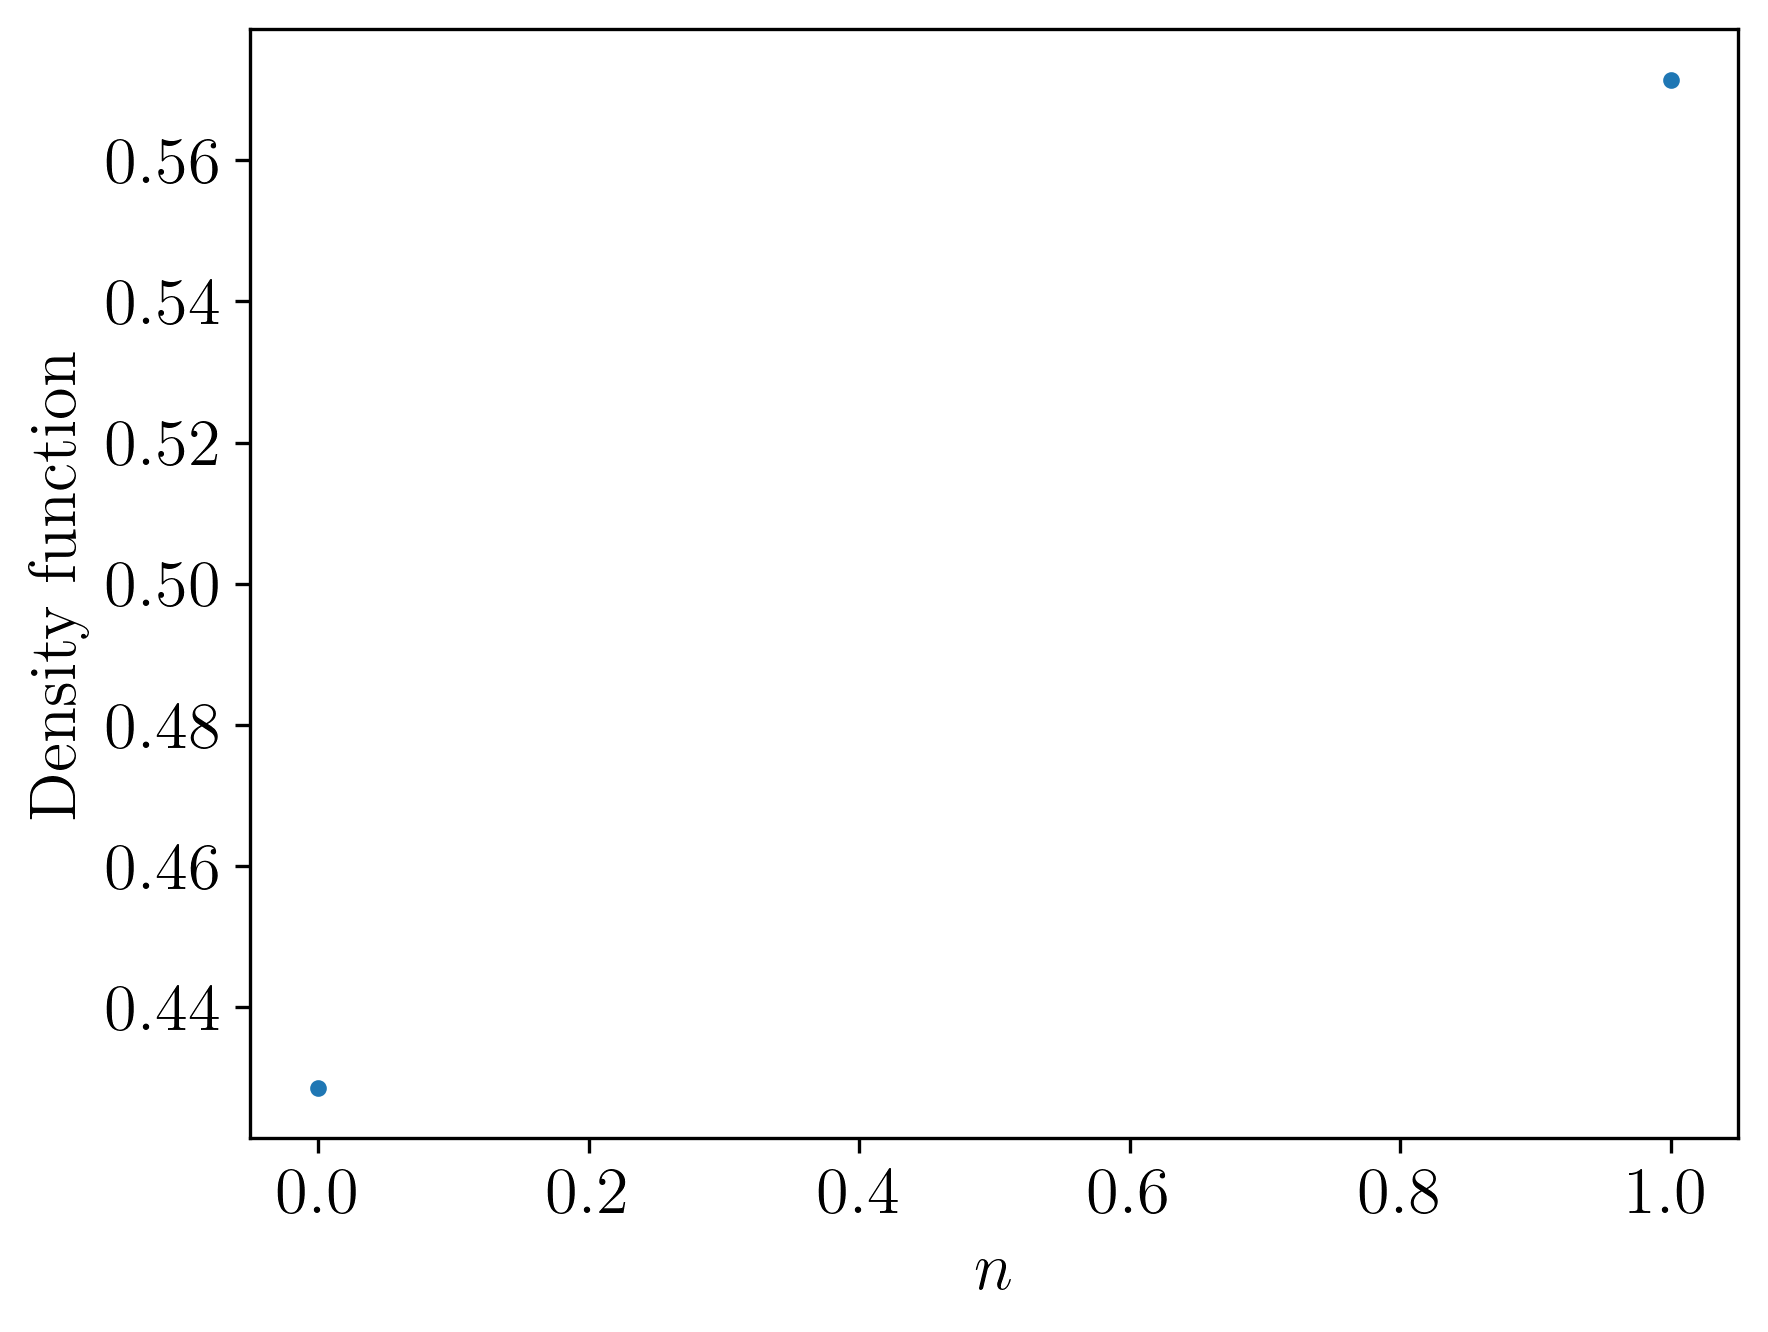
\includegraphics[width=0.5\linewidth]{./Section/Grundlegende Begriffe/Dichte Bernoulli.png}
\caption{Dichte einer $\Ber(4/7)$-Verteilung}
\end{figure}
Wir können diesen Plot auch modifizieren. Mittels
\begin{lstlisting}[numbers=left, numberstyle=\tiny\color{codegray}, firstnumber=6]
fig, ax = rv.plot_density(show=False)
ax.spines['top'].set_visible(False)
ax.spines['right'].set_visible(False)
ax.spines['bottom'].set_position('zero')
ax.spines['left'].set_position('zero')
ax.set_ylim(0)
ax.set_xticks([0, 1])
ax.set_yticks([3/7, 4/7], [r'$\frac{3}{7}$', r'$\frac{4}{7}$'])
plt.savefig('Dichte Bernoulli 2.png', dpi=300)
\end{lstlisting}

\newpage

erhalten wir
\begin{figure}[H]
\centering
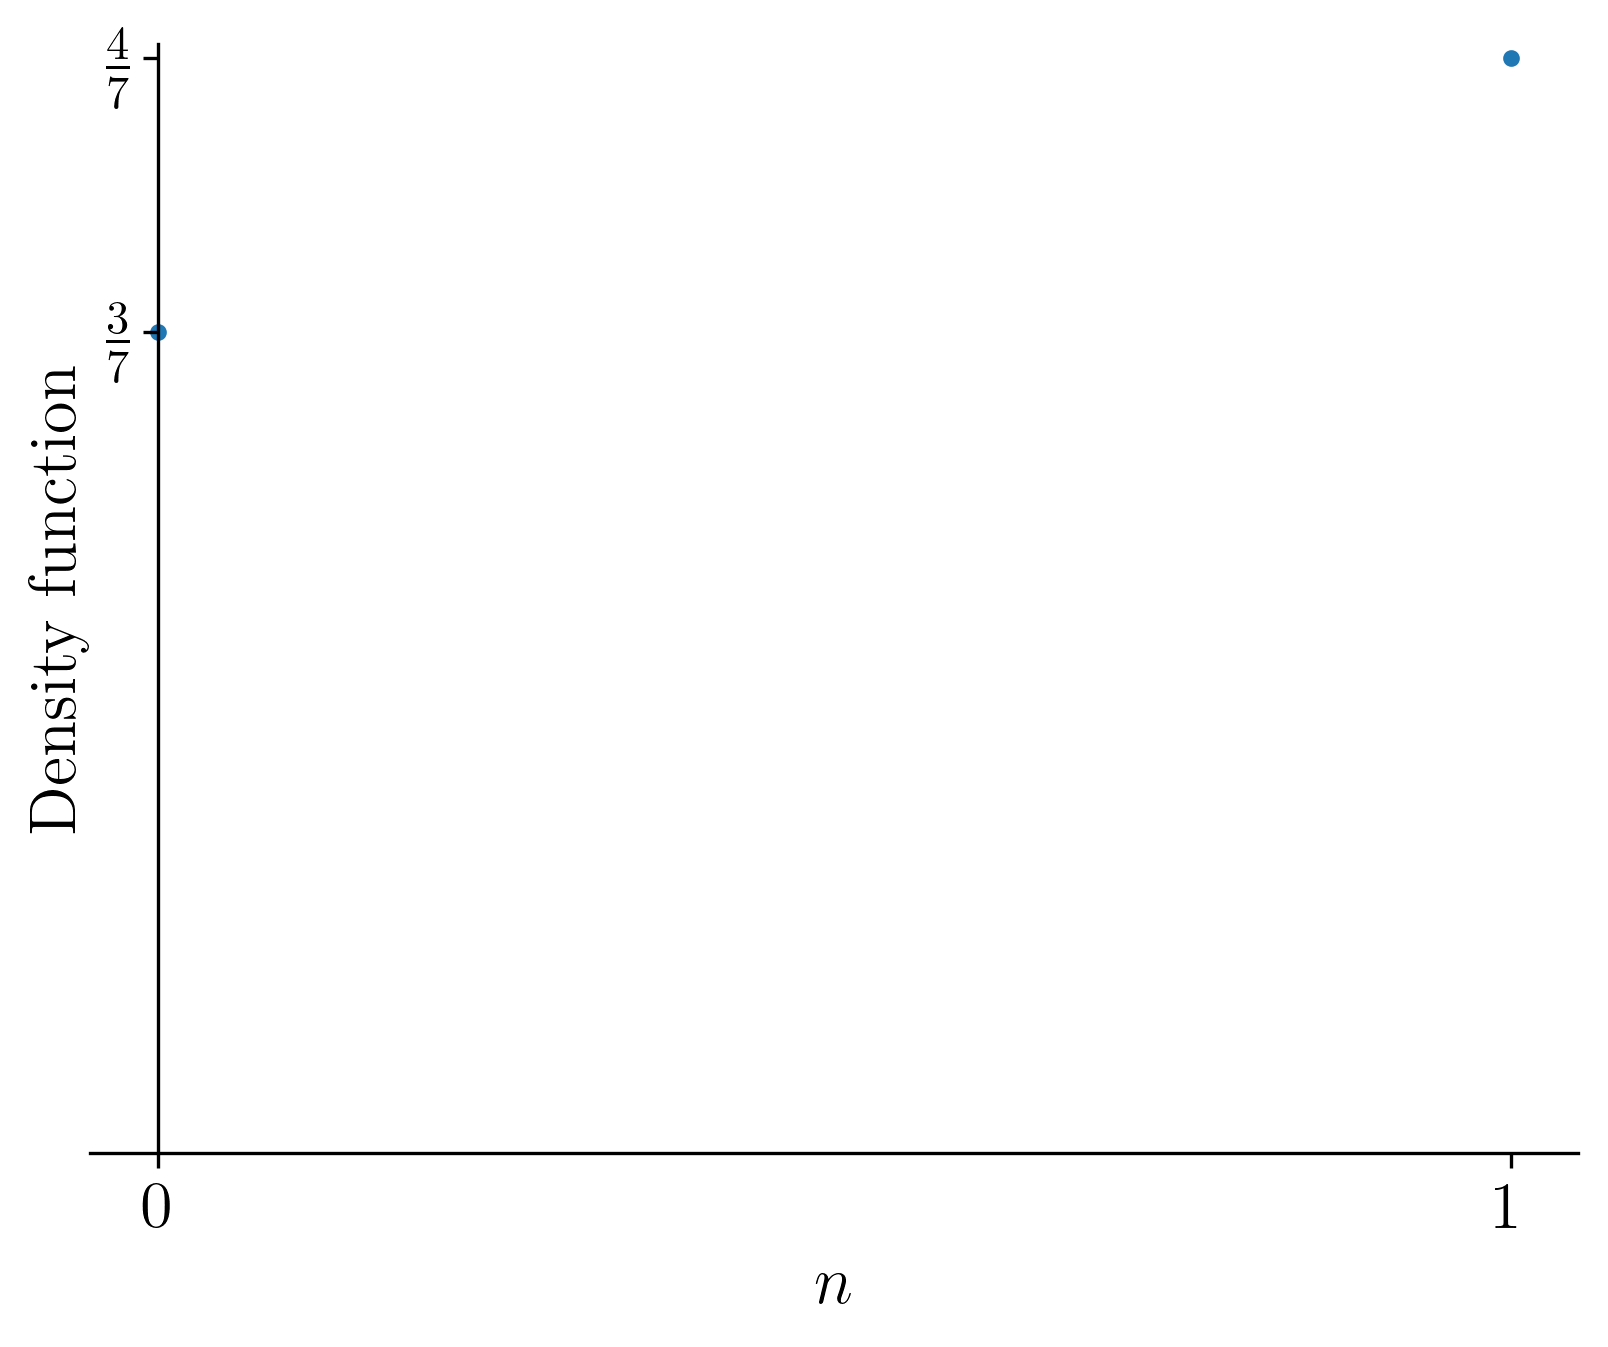
\includegraphics[width=0.5\linewidth]{./Section/Grundlegende Begriffe/Dichte Bernoulli 2.png}
\caption{Dichte einer $\Ber(4/7)$-Verteilung}
\end{figure}

\item Sei $X \sim \Bin(8, 2/3)$. Wir verwenden
\begin{lstlisting}[numbers=left, numberstyle=\tiny\color{codegray}]
k = sym.symbols('k', integer=True, nonnegative=True)
n = sym.Integer(8)
p = sym.Rational(2, 3)
density = sym.binomial(n, k) * p**k * (1 - p)**(n - k)
rv = RandomVariableDiscrete(density, k)
rv.plot_density()
\end{lstlisting}
und erhalten
\begin{figure}[H]
\centering
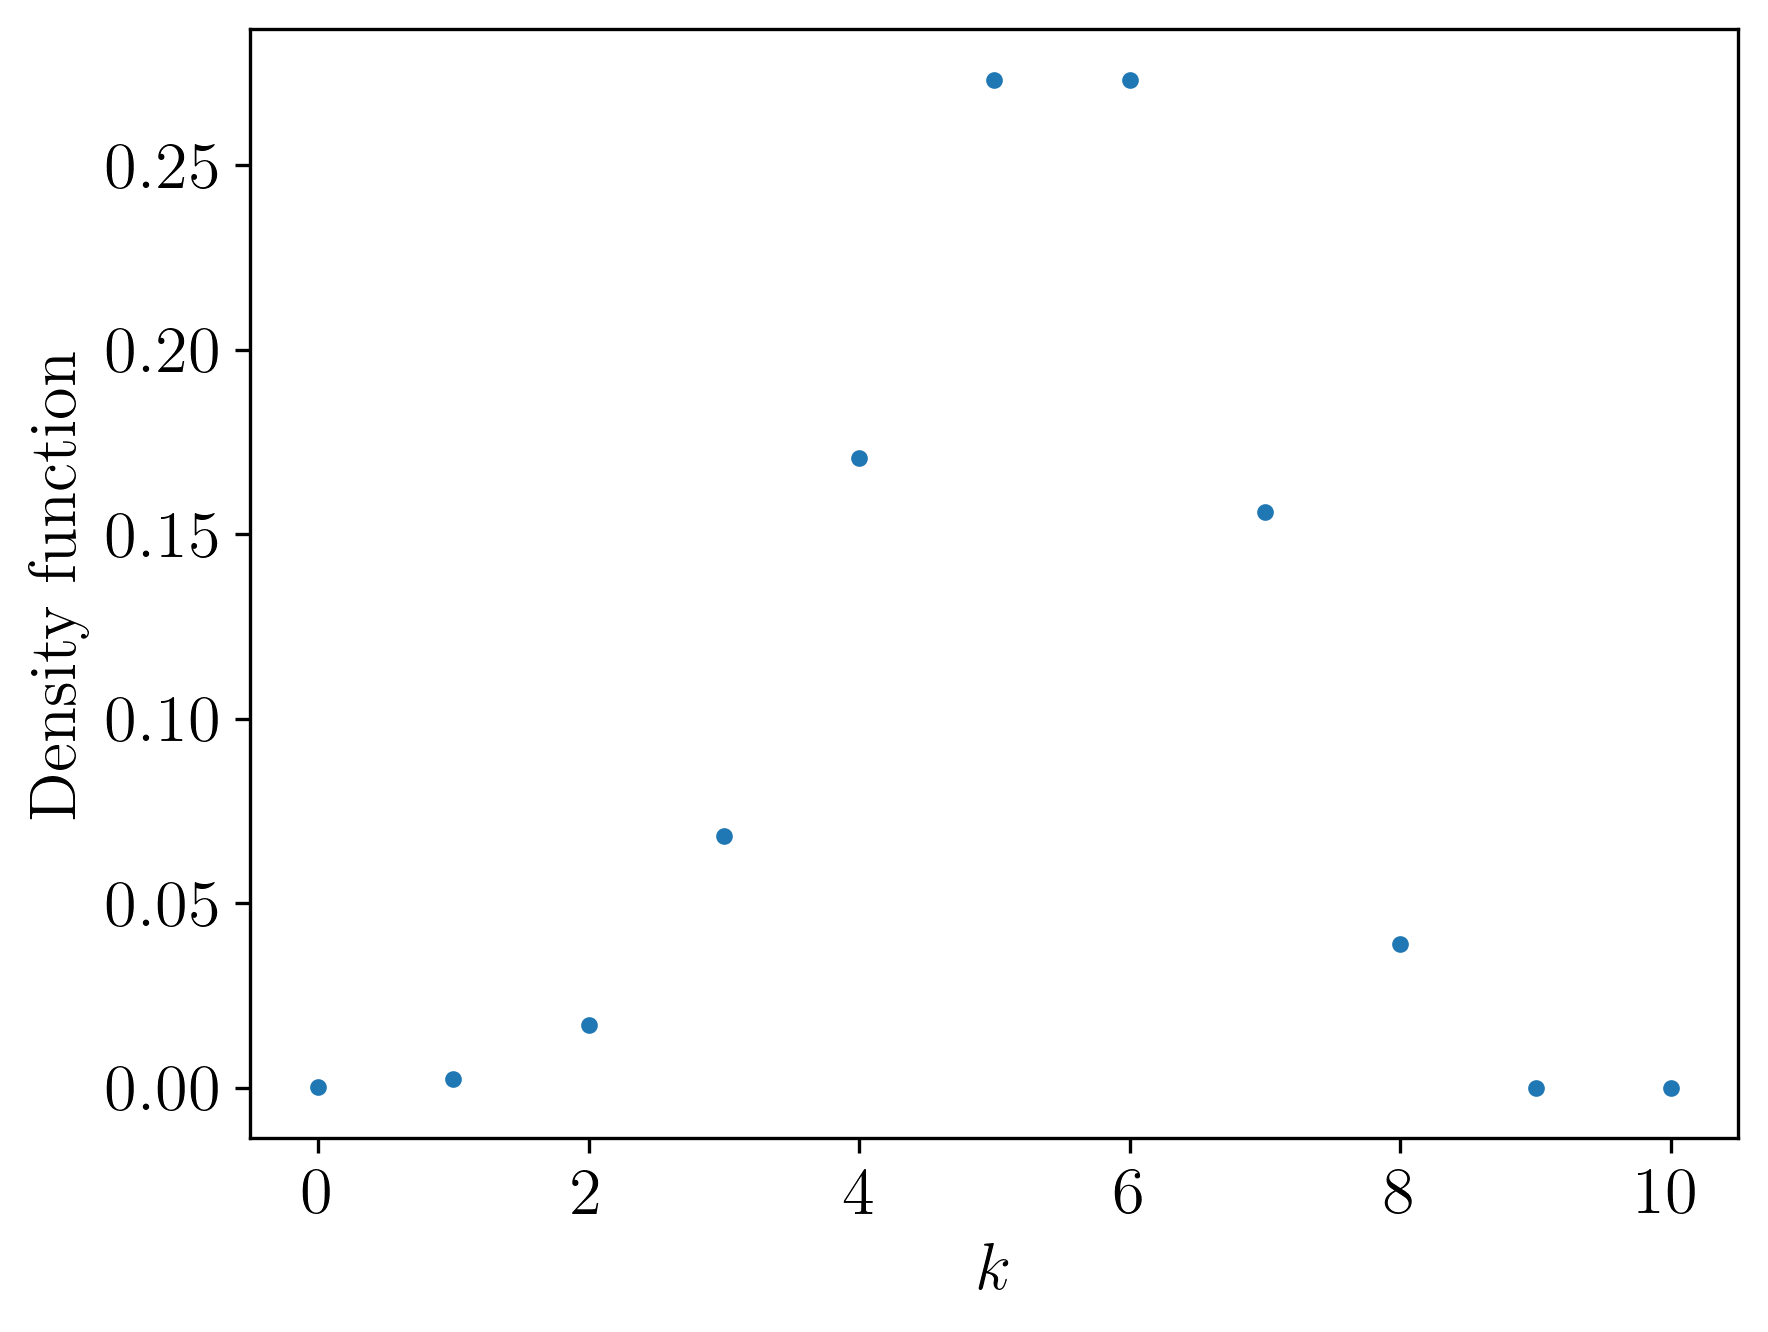
\includegraphics[width=0.5\linewidth]{./Section/Grundlegende Begriffe/Dichte Binomial.png}
\caption{Dichte einer $\Bin(8, 2/3)$-Verteilung}
\end{figure}
Dieser Plot ließe sich auch entsprechend verändern, worauf wir an dieser Stelle aber verzichten wollen.

\item Sei $X \sim \Nor(0, 1)$. Wir verwenden
\begin{lstlisting}[numbers=left, numberstyle=\tiny\color{codegray}]
mu = sym.Integer(0)
sigma = sym.Integer(1)
x = sym.symbols('x', real=True)
density = 1 / (sigma * sym.sqrt(2 * sym.pi)) * sym.exp(- (x - mu)**2 / (2 * sigma**2))
rv = RandomVariableContinuous(density, x)
rv.plot_density()
\end{lstlisting}
und erhalten
\begin{figure}[H]
\centering
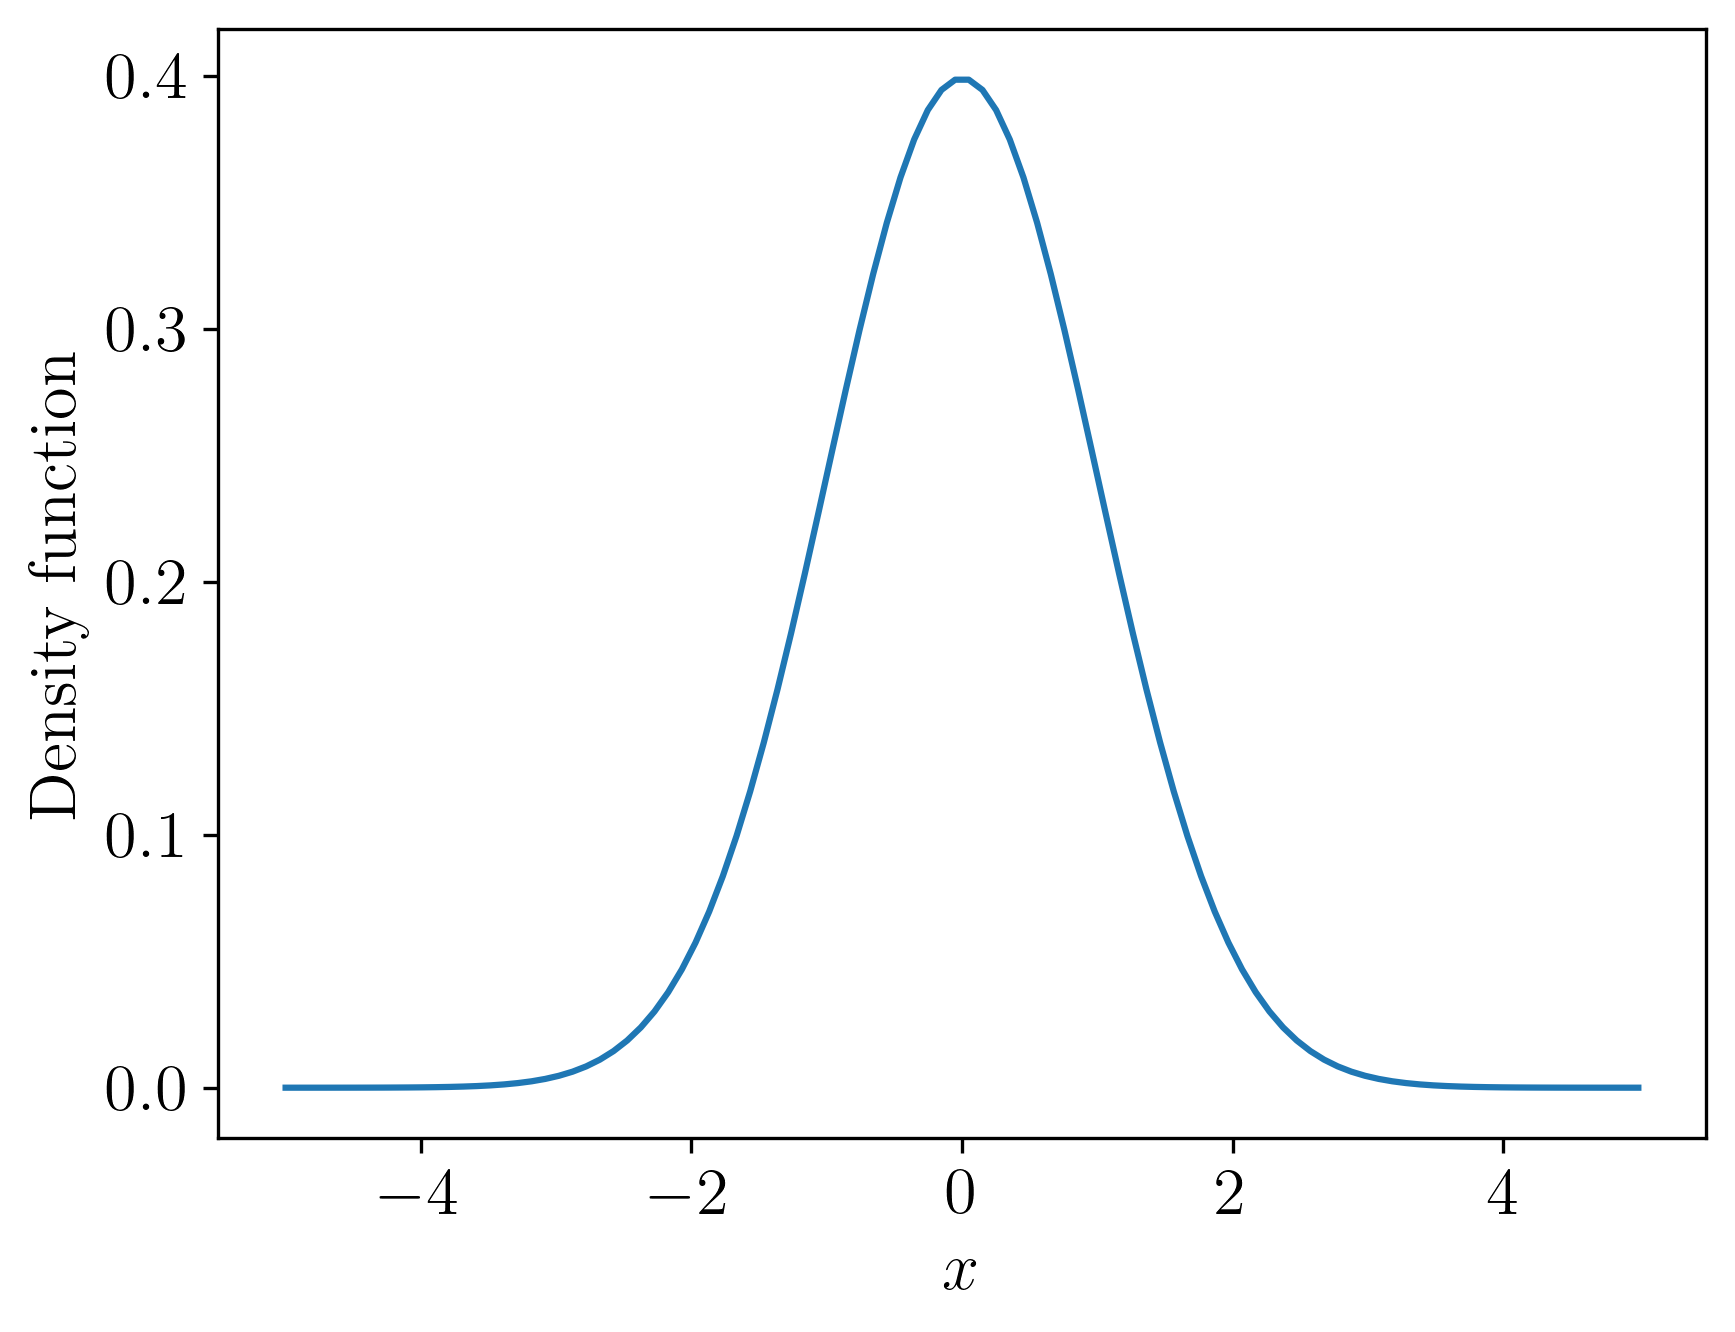
\includegraphics[width=0.5\linewidth]{./Section/Grundlegende Begriffe/Dichte Normal.png}
\caption{Dichte einer $\Nor(0, 1)$-Verteilung}
\end{figure}

\item Sei $X \sim \Exp(3)$. Diesen Plot wollen wir gleich etwas bearbeiten.
\begin{lstlisting}[numbers=left, numberstyle=\tiny\color{codegray}]
lamda = sym.Integer(3)
x = sym.symbols('x', real=True)
density = lamda * sym.exp(- lamda * x)
rv = RandomVariableContinuous(density, x, [sym.Integer(0), sym.oo])
fig, ax = rv.plot_density(numpoints=1000, show=False)
ax.spines['top'].set_visible(False)
ax.spines['right'].set_visible(False)
ax.spines['bottom'].set_position('zero')
ax.spines['left'].set_position('zero')
ax.set_xlim(-1, 4)
ax.set_ylim(0)
plt.show()
\end{lstlisting}
Wir erhalten
\begin{figure}[H]
\centering
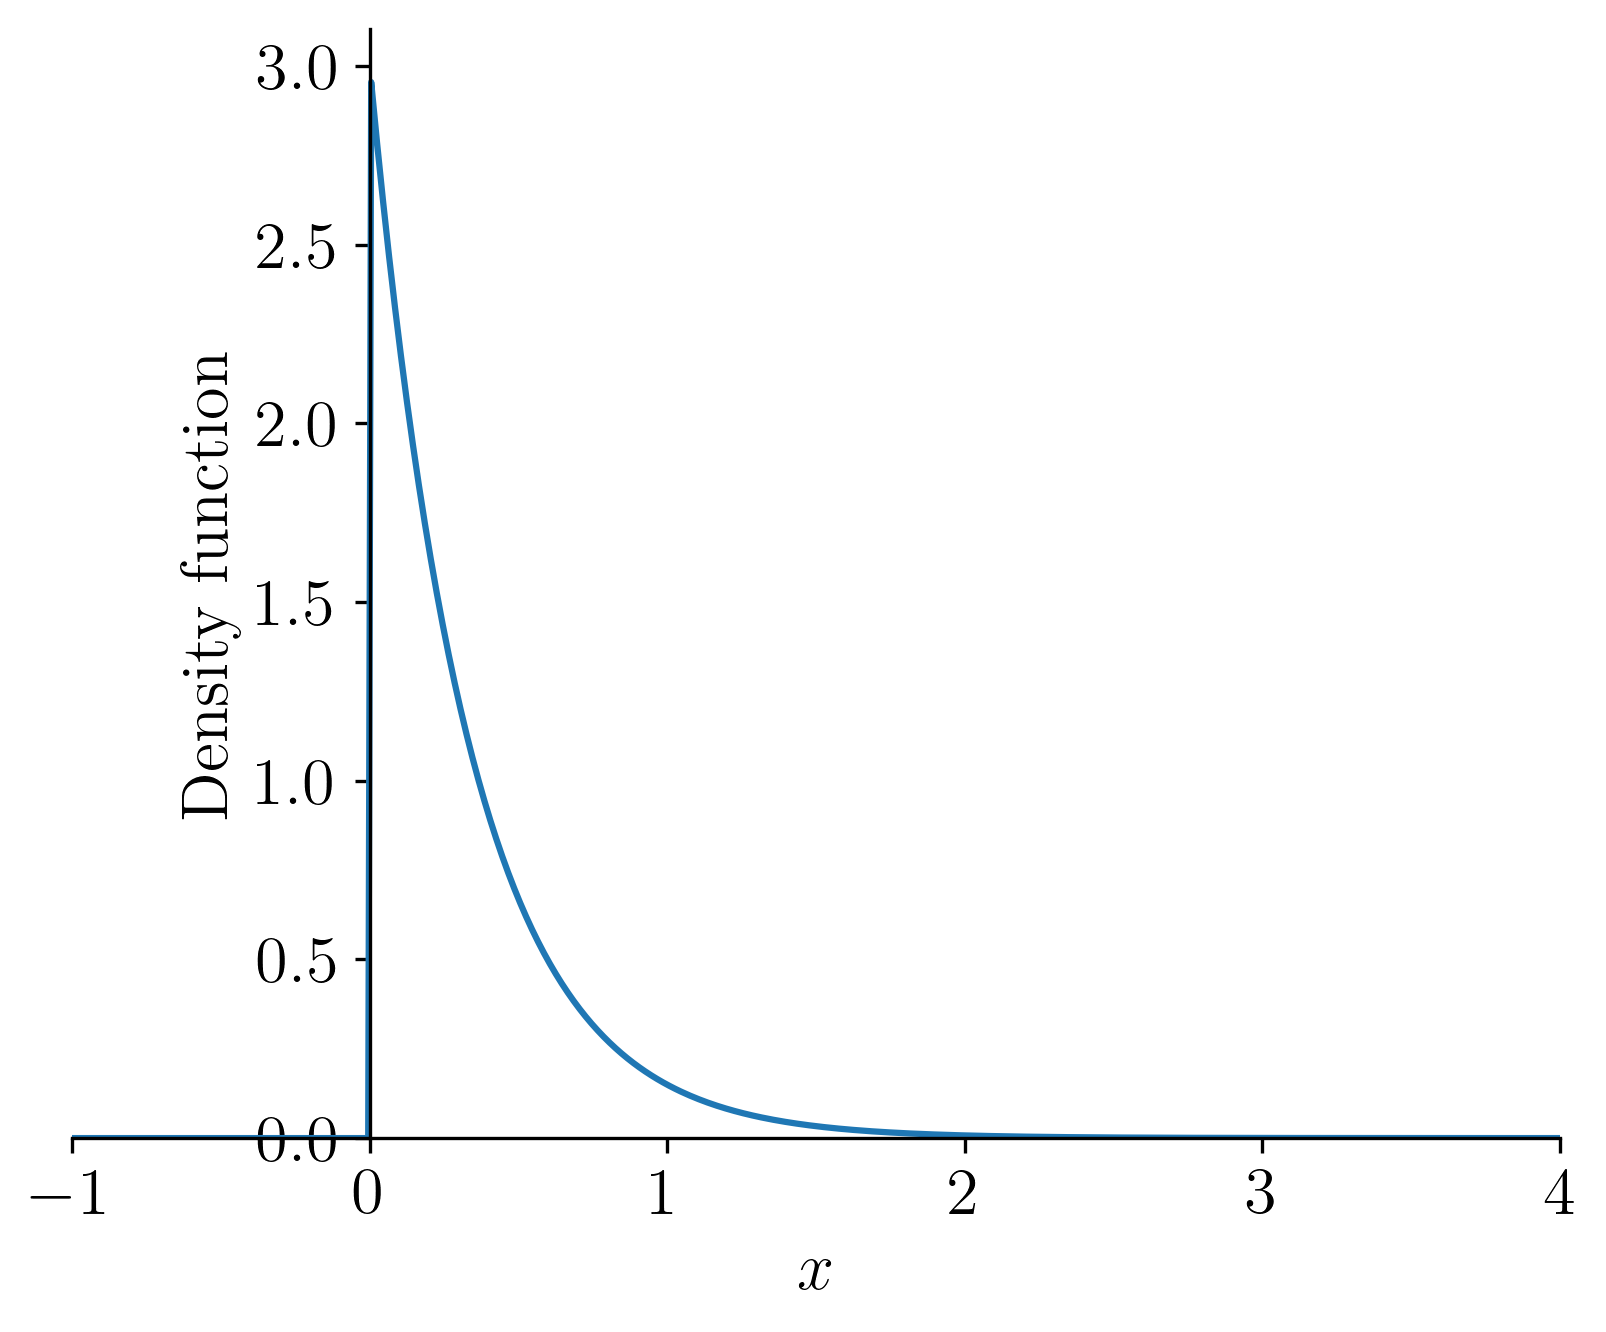
\includegraphics[width=0.5\linewidth]{./Section/Grundlegende Begriffe/Dichte Exponential.png}
\caption{Dichte einer $\Exp(3)$-Verteilung}
\end{figure}
\end{enumerate}
An dieser Stelle sei erwähnt, dass die Senkrechte um die Null mathematisch nicht schön ist. Die Dichte macht an dieser Stelle einen Sprung und diese Unterscheidung wäre in matplotlib theoretisch möglich, hätte aber zu einer unnötigen Spaghettifizierung des Codes geführt.
\end{Beispiel}

\newpage

Wir werden nun einen Satz betrachten und beweisen, mit dem wir Funktionen bezüglich des Bildmaßes integrieren können.

\begin{Satz}{(Maß und Bildmaß)}
\hypertarget{Satz:Maß_und_Bildmaß}{}Sei $(\Omega, \mathscr{A}, \mathbb{P})$ ein Wahrscheinlichkeitsraum und $X$ eine reelle Zufallsvariable. Weiter sei $f: \mathbb{R} \rightarrow \mathbb{R}$ eine messbare Funktion, so dass $f \circ X: \Omega \rightarrow \mathbb{R}$ $\mathbb{P}$-integrierbar ist. Dann gilt
\[\int f \d \mathbb{P}_X = \int f \circ X \d \mathbb{P}~.\]
\end{Satz}

\begin{Beweis}{}
Wir beweisen diesen Satz mittels algebraischer Induktion. Sei $B \in \mathscr{B}$ und $\indi_B$ die zugehörige Indikatorfunktion. Betrachte zunächst für $\omega \in \Omega$
\[\indi_B \circ X(\omega) = 1 \Leftrightarrow X(\omega) \in B \Leftrightarrow \omega \in X^{-1}(B)~.\]
Also gilt
\[\indi_B \circ X = \indi_{X^{-1}(B)}~.\]
Betrachte nun
\begin{align*}
\int \indi_B \d \mathbb{P}_X &= \int_B \d \mathbb{P}_X\\
&= \mathbb{P}_X(B)\\
&= \mathbb{P}(X^{-1}(B))\\
&= \int_{X^{-1}(B)} \d \mathbb{P}\\
&= \int \indi_{X^{-1}(B)} \d \mathbb{P}\\
&= \int \indi_B \circ X \d \mathbb{P}~.
\end{align*}
Sei nun $f$ eine Linearkombination von Indikatorfunktionen mit $(B_n)_{n \in \mathbb{N}_0} \subset \mathscr{B}$ und $(a_n)_{n \in \mathbb{N}_0} \subset \mathbb{R}$. Dann gilt dank Linearität des Integrals
\begin{align*}
\int \sum_{n \in \mathbb{N}_0} a_n \indi_{B_n} \d \mathbb{P}_X &= \sum_{n \in \mathbb{N}_0} a_n \int \indi_{B_n} \d \mathbb{P}_X~.
\intertext{Da dies nur Indikatorfunktionen sind, gilt nach dem ersten Schritt}
&= \sum_{n \in \mathbb{N}_0} a_n \int \indi_{B_n} \circ X \d \mathbb{P}\\
&= \int \sum_{n \in \mathbb{N}_0} a_n \indi_{B_n} \circ X \d \mathbb{P}~.
\end{align*}
Sei $f$ nun eine positive, messbare Funktion. Dann existiert eine monoton steigende Folge $(f_n)_{n \in \mathbb{N}_0}$ von Linearkombination von Indikatorfunktionen mit $\lim_{n \rightarrow \infty} f_n = f$. Dann gilt
\begin{align*}
\int f \d \mathbb{P}_X &= \int \lim_{n \rightarrow \infty} f_n \d \mathbb{P}_X~.
\intertext{Dank dem Satz von Lebesgue lassen sich Limes und Integration vertauschen und es gilt}
&= \lim_{n \rightarrow \infty} \int f_n \d \mathbb{P}_X~.
\intertext{Da dies Linearkombination von Indikatorfunktionen sind, gilt nach obigem}
&= \lim_{n \rightarrow \infty} \int f_n \circ X \d \mathbb{P}~.
\intertext{Nochmaliges Anwenden des Satzes von Lebesgue liefert}
&= \int \lim_{n \rightarrow \infty} f_n \circ X \d \mathbb{P}\\
&= \int f \circ X \d \mathbb{P}~.
\end{align*}
Sei nun $f$ nur noch eine messbare Funktion. Dann gibt es positive, messbare Funktion $f^+$ und $f^-$ mit $f = f^+ - f^+$ und es gilt
\begin{align*}
\int f \d \mathbb{P}_X &= \int f^+ - f^+ \d \mathbb{P}_X\\
&= \int f^+ \d \mathbb{P}_X - \int f^- \d \mathbb{P}_X~.
\intertext{Da dies positive messbare Funktionen sind, folgt dank obigem}
&= \int f^+ \circ X \d \mathbb{P} - \int f^- \circ X \d \mathbb{P}\\
&= \int f^+ \circ X - f^- \circ X \d \mathbb{P}\\
&= \int (f^+ - f^+) \circ X \d \mathbb{P}\\
&= \int f \circ X \d \mathbb{P}~.
\end{align*}
Die Aussage gilt somit für alle messbaren Funktionen und wir sind fertig.
\end{Beweis}
\vspace*{\baselineskip}

Nun werden wir einen Satz beweisen, der es uns erlaubt Funktionen, die wir bezüglich des Bildmaßes integrieren wollen auf einem einfacheren Wege mithilfe der Dichtefunktion zu integrieren.

\begin{Satz}{(Dichtesatz)}
\hypertarget{Satz:Dichtesatz}{}Sei $(\Omega, \mathscr{A}, \mathbb{P})$ ein Wahrscheinlichkeitsraum und $X$ eine reelle Zufallsvariable mit Lebesgue-Dichte $\varphi$. Weiter sei $f: \mathbb{R} \rightarrow \mathbb{R}$ eine Funktion, sodass $f \cdot \varphi$ $\lambda$-integrierbar ist. Dann gilt
\[\int f \d \mathbb{P}_X = \int f \varphi \d \lambda~.\] 
Eine analoge Aussage gilt für das Zählmaß.
\end{Satz}

\begin{Beweis}{}
Wir beweisen diesen Satz mittels algebraischer Induktion. Sei $B \in \mathscr{B}$ und $\indi_B$ die zugehörige Indikatorfunktion. Betrachte
\begin{align*}
\int \indi_B \d \mathbb{P}_X &= \mathbb{P}_X(B)~.
\intertext{Da $\varphi$ eine $\lambda$-Dichte des Maßes $\mathbb{P}_X$ ist, folgt direkt aus der \hyperlink{Def:Dichtefunktion}{\blue{Definition der Dichtefunktion}}}
&= \int \indi_B \varphi \d \lambda~.
\end{align*}
Sei nun $f$ eine Linearkombination von Indikatorfunktionen mit $(B_n)_{n \in \mathbb{N}_0} \subset \mathscr{B}$ und $(a_n)_{n \in \mathbb{N}_0} \subset \mathbb{R}$. Dann gilt dank Linearität des Integrals
\begin{align*}
\int \sum_{n \in \mathbb{N}_0} a_n \indi_{B_n} \d \mathbb{P}_X &= \sum_{n \in \mathbb{N}_0} a_n \int \indi_{B_n} \d \mathbb{P}_X~.
\intertext{Da dies nur Indikatorfunktionen sind, gilt nach dem ersten Schritt}
&= \sum_{n \in \mathbb{N}_0} a_n \int \indi_{B_n} \varphi \d \lambda\\
&= \int \sum_{n \in \mathbb{N}_0} a_n \indi_{B_n} \varphi \d \lambda\\
&= \int \left( \sum_{n \in \mathbb{N}_0} a_n \indi_{B_n} \right) \varphi \d \lambda~.
\end{align*}
Sei $f$ nun eine positive, messbare Funktion. Dann existiert eine monoton steigende Folge $(f_n)_{n \in \mathbb{N}_0}$ von Linearkombinationen von Indikatorfunktionen mit $\lim_{n \rightarrow \infty} f_n = f$. Dann gilt
\begin{align*}
\int f \d \mathbb{P}_x &= \int \lim_{n \rightarrow \infty} f_n \d \mathbb{P}_X~.
\intertext{Dank dem Satz von Lebesgue lassen sich Limes und Integration vertauschen und es gilt}
&= \lim_{n \rightarrow \infty} \int f_n \d \mathbb{P}_X~.
\intertext{Da dies Linearkombinationen von Indikatorfunktionen sind, gilt nach obigem}
&= \lim_{n \rightarrow \infty} \int f_n \varphi \d \lambda~.
\intertext{Nochmaliges Anwenden des Satzes von Lebesgue liefert}
&= \int \lim_{n \rightarrow \infty} f_n \varphi \d \lambda\\
&= \int f \varphi \d \lambda~.
\end{align*}
Sei nun $f$ nur noch eine messbare Funktion. Dann gibt es positive, messbare Funktion $f^+$ und $f^-$ mit $f = f^+ - f^+$ und es gilt
\begin{align*}
\int f \d \mathbb{P}_X &= \int f^+ - f^- \d \mathbb{P}_X\\
&= \int f^+ \d \mathbb{P}_X - \int f^- \d \mathbb{P}_X~.
\intertext{Da dies positive messbare Funktionen sind, folgt dank obigem}
&= \int f^+ \varphi \d \lambda - \int f^- \varphi \d \lambda\\
&= \int f^+ \varphi - f^- \varphi \d \lambda\\
&= \int \left( f^+ - f^- \right) \varphi \d \lambda\\
&= \int f \varphi \d \lambda~.
\end{align*}
Die Aussage gilt somit für alle messbaren Funktionen und wir sind fertig.
\end{Beweis}
\vspace*{\baselineskip}

\newpage

Die Kombination dieser beiden Sätze liefert das folgende Korollar. Dies liefert uns eine einfach Möglichkeit Maßintegrale mit bekannten Werkzeugen zu Riemann- beziehungsweise Lebesgue-Integralen und Reihen zu berechnen.

\begin{Korollar}{(Dichtekorollar)}
\hypertarget{Kor:Dichtekorollar}{}Sei $(\Omega, \mathscr{A}, \mathbb{P})$ ein Wahrscheinlichkeitsraum und $X$ eine reelle Zufallsvariable mit Lebesgue-Dichte $\varphi$. Weiter sei $f: \mathbb{R} \rightarrow \mathbb{R}$ eine messbare Funktion, so dass $f \circ X: \Omega \rightarrow \mathbb{R}$ $\mathbb{P}$-integrierbar und $f \cdot \varphi$ $\lambda$-integrierbar ist. Dann gilt
\[\int f \circ X \d \mathbb{P} = \int f \varphi \d \lambda~.\]
Eine analoge Aussage gilt für das Zählmaß.
\end{Korollar}

\begin{Beweis}{}
Wir verbinden die Aussagen der vorangegangenen Sätze. Betrachte mit dem \hyperlink{Satz:Maß_und_Bildmaß}{\blue{Satz von Maß und Bildmaß}}
\begin{align*}
\int f \circ X \d \mathbb{P} &= \int f \d \mathbb{P}_X\\
&= \int f \varphi \d \lambda~,
\end{align*}
dank dem gerade bewiesenen \hyperlink{Satz:Dichtesatz}{\blue{Dichtesatz}}.
\end{Beweis}
%\vspace*{\baselineskip}

\begin{Bemerkung}{(Dichtekorollar Summenform)}
Wir können das obige \hyperlink{Kor:Dichtekorollar}{\blue{Dichtkorollar}} in die Form für diskrete Zufallsvariablen schreiben. Sei $(\Omega, \mathscr{A}, \mathbb{P})$ ein Wahrscheinlichkeitsraum und $X$ eine diskrete Zufallsvariable mit Zähldichte $\varphi$. Dann gilt für $f : \mathbb{N}_0 \rightarrow \mathbb{R}$
\begin{align*}
\int f \circ X \d \mathbb{P} &= \int f \varphi \d \#\\
&= \sum_{n \in \mathbb{N}_0} f(n) \varphi(n)~.
\end{align*}
Analog gilt dies auch für finite Zufallsvariablen.\\

Sei $X$ nun eine stetige Zufallsvariable mit Dichte $\varphi$. Ist $f \varphi$ für stetige Zufallsvariablen sogar Riemann-integrierbar, so können wir die Integrale wie gewohnt mit dem Hauptsatz berechnen. Diese Voraussetzung nehmen wir im Folgenden häufig implizit an.
\end{Bemerkung}

Wollen wir also die Funktion einer Zufallsvariable bezüglich des Wahrscheinlichkeitsmaßes $\mathbb{P}$ berechnen, so genügt es entsprechende Lebesgue-Integral oder die Summe zu berechnen, falls diese existiert. Wir können nun eine Methode definieren, die genau dieses Korollar anwendet.

\begin{Code}{(\lstinline|integrate_random_variable|)}
\hypertarget{Code:Integrate}{}Ziel dieser Methode ist es Integrale von $f(X)$ zu bestimmen. Sei  $X$ eine reelle Zufallsvariable mit Dichte $\varphi$ und $f$ eine Funktion, die wir mit \lstinline|expr| bezeichnen. Da sich das Zähl- und Lebesgue-Maß grundlegend in ihrer Berechnung unterscheiden, ist diese Methode für jeden Typ von Zufallsvariable separat definiert.
\begin{enumerate}[label=(\roman*)]
\item Für finite Zufallsvariablen gilt
\begin{lstlisting}
def integrate_random_variable(self, expr, lower=-sym.oo, upper=sym.oo):
    integral = sym.Integer(0)
    for key in self.density.keys():
        if key >= lower and key <= upper:
            integral += expr.subs(self.variable, key) * self.density[key]
    integral = sym.simplify(integral)
    return integral
\end{lstlisting}

\newpage

Wir lassen hier untere und obere Grenzen für die Summation zu, welche standardmäßig $- \infty$ und $\infty$ sind. Da die Dichte einer finiten Zufallsvariable aus einem Dictionary besteht, können wir über deren Schlüssel iterieren. Ist der Schlüssel innerhalb des Integrationsintervalls, ersetzen wir mithilfe der \lstinline|subs|-Methode in jeder Iteration die Variable der Funktion durch den entsprechenden Schlüssel und multiplizieren dies mit der Wahrscheinlichkeit diesen Wert zu erhalten, was \lstinline|self.density[key]| entspricht. Zuletzt lassen wir SymPy diesen Ausdruck vereinfachen und anschließend ausgeben.

\item Für diskrete Zufallsvariablen gilt
\begin{lstlisting}
def integrate_random_variable(self, expr, lower=sym.Integer(0), upper=sym.oo):
    lower = sym.Max(lower, self.supp[0])
    upper = sym.Min(upper, self.supp[1])
    integral = sym.summation(expr * self.density, (self.variable, lower, upper)).doit()
    integral = RandomVariable.clean_piecewise(integral)
    integral = sym.simplify(integral)
    return integral
\end{lstlisting}
Wir lassen hier untere und obere Grenzen für die Summation zu, welche standardmäßig $0$ und $\infty$ sind. Diese Summationsgrenzen werden dann noch mit den Grenzen für die Werte der Zufallsvariable verarbeitet. Mithilfe von SymPy bilden wir die Summe aus Funktion und Dichte  und summieren von der unteren bis zur oberen Grenze. Als nächstes wird aus der Hauptklasse die \lstinline|clean_piecewise|-Funktion aufgerufen. Diese überprüft einen Ausdruck, ob dieser zur SymPy \lstinline|Piecewise|-Klasse gehört. Dies ist das SymPy Objekt für stückweise definiert Funktionen. Ist der Ausdruck aus dieser Klasse, so nimmt die Funktion immer den ersten Zweig dieser Funktion, da dieser meist das gesuchte Ergebnis ist und gibt eine Warnung in der Konsole aus. Sollte man nicht wollen, dass stückweise Funktionen gekürzt werden, so kann man die \lstinline|no_chopping|-Funktion aufrufen. Es ist zu beachten, dass dann die meisten Funktionen nicht mehr funktionieren, da SymPy mit stückweisen Funktionen nicht richtig weiterrechnen kann. Zum Schluss wird wieder versucht das Ergebnis zu vereinfachen.

\item Für stetige Zufallsvariablen gilt
\begin{lstlisting}
def integrate_random_variable(self, expr, lower=-sym.oo, upper=sym.oo):
    lower = sym.Max(lower, self.supp[0])
    upper = sym.Min(upper, self.supp[1])
    integral = sym.integrate(expr * self.density, (self.variable, lower, upper)).doit()
    integral = RandomVariable.clean_piecewise(integral)
    integral = sym.simplify(integral)
    return integral
\end{lstlisting}
Wir lassen auch hier obere und untere Grenzen zu, welche standardmäßig auf $\infty$ und $- \infty$ gesetzt werden. Da wir für die Dichten von stetigen Zufallsvariablen die Indikatorfunktionen weggelassen haben, müssen wir diese in einem ersten Schritt mit dem Träger der Dichte vergleichen. Anschließend integrieren wir mit SymPy das Produkt aus Funktion und Dichte von der unteren zur oberen Grenze. Nach der Entfernung von stückweisen Funktionen wird dies wieder vereinfacht und ausgegeben.
\end{enumerate}

Der besonders elegante Teil besteht darin, dass wir in der Aufforderung für die Berechnung quasi die maßtheoretische Integration einer Zufallsvariable verwenden können, da der Code das Dichtekorollar automatisch anwendet und die Dichtefunktion dazu multipliziert.
\end{Code}

\newpage

Wir können nun versuchen mit der obigen Methode eine Funktion einer Zufallsvariable zu integrieren.

\begin{Beispiel}{(Funktionen von Zufallsvariablen)}
\begin{enumerate}[label=(\roman*)]
\item Sei $X$ eine finite Zufallsvariable mit
\begin{align*}
\mathbb{P}(X = 1) &= p\\
\mathbb{P}(X = 2) &= q\\
\mathbb{P}(X = 3) &= 1 - p - q\\
\end{align*}
mit $p, q \in (0, 1)$. Wir berechnen nun mit $E = \{ 1, 2, 3 \}$
\begin{align*}
\int X^2 + 2 X \d \mathbb{P} &= \sum_{n \in E} (n^2 + 2 n) \mathbb{P}(X = n)\\
&= (1^2 + 2 \cdot 1) \mathbb{P}(X = 1) + (2^2 + 2 \cdot 2) \mathbb{P}(X = 2) + (3^2 + 2 \cdot 3) \mathbb{P}(X = 3)\\
&= (1 + 2) p + (4 + 4) q + (9 + 6) (1 - p - q)\\
&= 3 p + 8 q + 15 - 15 p - 15 q\\
&= 15 - 12 p - 7 q
\end{align*}
Dies können wir nun folgendermaßen mit der oben definierten Funktion berechnen lassen.
\begin{lstlisting}[numbers=left, numberstyle=\tiny\color{codegray}]
n = sym.Symbol('n', integer=True, positive=True)
p, q = sym.symbols('p, q', real=True, positive=True)
density = {1: p, 2: q, 3: 1 - p - q}
rv = RandomVariableFinite(density, n)
polynom = rv.integrate_random_variable(n**2 + 2 * n)
\end{lstlisting}
Als Ergebnis erhalten wir \lstinline|-12*p - 7*q + 15|.

\item Sei $X \sim \Exp(\lambda)$ mit $\lambda > 0$ exponentialverteilt. Betrachte nun mit dem \hyperlink{Kor:Dichtekorollar}{\blue{Dichtekorollar}}
\begin{align*}
\int \sin(X) \d \mathbb{P} &= \int_{-\infty}^\infty \sin(x) \lambda \exp(- \lambda x) \indi_{[0, \infty)}(x) \d x\\
&= \lambda \int_0^\infty \sin(x) \exp(- \lambda x) \d x~.
\end{align*}
Weiter betrachten wir das Integral
\begin{align*}
\alpha &= \int_0^\infty \sin(x) \exp(- \lambda x) \d x
\intertext{Mit partieller Integration erhalten wir}
&= \left[ \frac{1}{\lambda} \sin(x) \exp(- \lambda x) \right]_0^\infty + \frac{1}{\lambda} \int_0^\infty \cos(x) \exp(- \lambda x) \d x\\
&= \left[ 0 - 0 \right] + \frac{1}{\lambda} \int_0^\infty \cos(x) \exp(- \lambda x) \d x\\
&= \frac{1}{\lambda} \int_0^\infty \cos(x) \exp(- \lambda x) \d x~.
\displaybreak
\intertext{Nochmal partielle Integration liefert}
&= \left[ - \frac{1}{\lambda^2} \cos \exp(- \lambda x) \right]_0^\infty - \frac{1}{\lambda^2} \int_0^\infty \sin(x) \exp(- \lambda x) \d x\\
&= \left[ - 0 + \frac{1}{\lambda^2} \right] - \frac{1}{\lambda^2} \int_0^\infty \sin(x) \exp(- \lambda x) \d x\\
&= \frac{1}{\lambda^2} - \frac{1}{\lambda^2} \alpha~.
\end{align*}
Zusammengefasst ist also
\begin{align*}
\alpha &= \frac{1}{\lambda^2} - \frac{1}{\lambda^2} \alpha~.
\intertext{Umformen liefert}
(\lambda^2 + 1) \alpha &= 1\\
\alpha &= \frac{1}{\lambda^2 + 1}~.
\end{align*}
Damit ist dann insgesamt
\[\int \sin(X) \d \mathbb{P} = \frac{\lambda}{\lambda^2 + 1}~.\]
Dies können wir folgendermaßen berechnen lassen
\begin{lstlisting}[numbers=left, numberstyle=\tiny\color{codegray}]
x = sym.Symbol('x', real=True)
lamda = sym.Symbol('lambda', real=True, positive=True)
density = lamda * sym.exp(- lamda * x)
rv = RandomVariableContinuous(density, x, [sym.Integer(0), sym.oo])
sine = rv.integrate_random_variable(sym.sin(x))
\end{lstlisting}
Wir erhalten analog \lstinline|lambda/(lambda**2 + 1)|.

\item Sei $X \sim \Nor(0, 1)$ standardnormalverteilt. Wir können mit dieser Methode beispielsweise
\[\int \log(X) \d \mathbb{P}\]
berechnen. Es ist zu beachten, dass $\log$ den natürlichen Logarithmus bezeichnet.
\begin{lstlisting}[numbers=left, numberstyle=\tiny\color{codegray}]
x = sym.Symbol('x', real=True)
density = 1 / sym.sqrt(2 * sym.pi) * sym.exp(- x**2 / 2)
rv = RandomVariableContinuous(density, x)
natural_logarithm = rv.integrate_random_variable(sym.log(x))
\end{lstlisting}
Wir erhalten
\begin{align*}
\int \log(X) \d \mathbb{P} &= - \frac{\log{\left(2 \right)}}{2} - \frac{\gamma}{2} + \frac{i \pi}{2}\\
&= \frac{1}{2} \left( - \log(2) - \gamma + i \pi \right)~.
\end{align*}
Dies ist ein sehr interessantes Ergebnis, da hier einige wichtige mathematische Konstanten auftauchen. Die eulersche Zahl $e$ implizit im natürliche Logarithmus von $2$, die Euler–Mascheroni-Konstante $\gamma$, die komplexe Einheit $i$ und die Kreiszahl $\pi$. Dies können wir leider nicht auf elementare Weise nachrechnen.
\end{enumerate}
Wir werden später in vielen Funktionen diese \lstinline|integrate_random_variable|-Methode benötigen.
\end{Beispiel}

\newpage

Mit dieser Integrationsmethode können wir nun die \lstinline|_is_density|-Methode definieren, welche bei der \hyperlink{Code:Initialisierung}{\blue{Initialisierung einer Zufallsvariable}} aufgerufen wird.

\begin{Code}{(\lstinline|_is_density|)}
Mit dieser Methode überprüfen wir, ob die Wahrscheinlichkeit des gesamten Raumes gleich eins ist. Dies ist folgendermaßen implementiert
\begin{lstlisting}
def _is_density(self):
    total = self.integrate_random_variable(sym.Integer(1))
    if not total.equals(sym.Integer(1)):
        print('WARNING: Density not standardized!')
    return total
\end{lstlisting}
Mithilfe der gerade definieren Integrationsmethode wird über die Einsfunktion integriert. Wir bilden also im stetigen Fall
\begin{align*}
\int_\mathbb{R} 1 \varphi(x) \d x &= \int_\mathbb{R} \varphi(x)  \d x\\
&= \mathbb{P}_X(\mathbb{R})~.
\end{align*}
Für ein Wahrscheinlichkeitsmaß war dies nach \hyperlink{Def:Maß}{\blue{Definition}} eins. Streng genommen müssten wir noch nachrechnen, dass die Dichtefunktion überall nicht-negativ ist. Hierfür gibt es leider keine einfache und effiziente Methode, weshalb diese Überprüfung nicht stattfindet. Diese Methode dient allgemein nur dazu, dem Nutzer offensichtliche Fehler bei der Eingabe der Dichte mitzuteilen. Ist die Dichte nicht normiert, so wird eine entsprechende Warnung in der Konsole ausgegeben. Sollte man diese Überprüfung unterdrücken wollen, so muss man bei der Definition der Zufallsvariable zusätzlich \lstinline|force_denisty=True| übergeben, was die gesamte Überprüfung überspringt. Hier wurde bewusst kein Python-Fehler verwendet. Dieser würde das Programm sofort beenden und es gibt leider Zufallsvariablen, deren Dichten SymPy nicht zu eins vereinfachen kann. Sei dazu $X \sim \Log(p)$ mit $p \in (0, 1)$ logarithmischverteilt. Die Dichte ist gegeben durch
\[\varphi(n) = - \frac{p^n}{n} \frac{1}{\log(1 - p)}\]
für alle $n \in \mathbb{N}$. Wir können daraus nun ein \lstinline|RandomVariable|-Objekt machen.
\begin{lstlisting}[numbers=left, numberstyle=\tiny\color{codegray}]
p = sym.Symbol('p', real=True, positive=True)
n = sym.Symbol('n', integer=True, nonnegative=True)
density = - p**n / n * 1 / sym.log(1 - p)
rv = RandomVariableDiscrete(density, n, supp=[sym.Integer(1), sym.oo])
\end{lstlisting}
Wir erhalten nun die Meldung \lstinline|WARNING: Density not standardized!|. Dies liegt vermutlich daran, dass SymPy die Summe nicht zusammenfassen möchte, da wir nicht festlegen können, dass $p < 1$ ist.
\end{Code}

Da uns Dichtefunktionen die Arbeit erleichtern, wollen wir nun allgemein wissen, wann eine solche Funktion existiert. Für diesen zentralen Satz der Maßtheorie benötigen wir zunächst die folgende

\begin{Definition}{(Nullmenge)}
Sei $(\Omega, \mathscr{A}, \mu)$ ein Maßraum und $A \in \mathscr{A}$ eine Menge. Gilt
\[\mu(A) = 0~,\]
so ist $A$ eine \textit{$\mu$-Nullmenge} oder nur \textit{Nullmenge}.
\end{Definition}

\newpage

Nun können wir einige typische Beispiele für Nullmengen betrachten.

\begin{Beispiel}{(Nullmenge)}
\hypertarget{Bsp:Nullmenge}{}
\begin{enumerate}[label=(\roman*)]
\item Betrachten wir $(\Omega, \mathscr{A}, \delta_{\{\omega\}})$ mit einem $\omega \in \Omega$, so ist jede Menge $A \in \mathscr{A}$ mit $\omega \notin A$ eine $\delta_{\{\omega\}}$-Nullmenge.

\item Betrachten wir $(\mathbb{R}, \mathscr{B}, \lambda)$, so ist jede Einpunktmenge eine Nullmenge. Sei dazu $x \in \mathbb{R}$. Dann gilt
\begin{align*}
\lambda(\{x\}) &= \lambda([x, x])\\
&= x - x\\
&= 0~.
\end{align*}

\item Betrachte wieder $(\mathbb{R}, \mathscr{B}, \lambda)$. Dann ist jede abzählbare Menge eine Nullmenge. Sei nun $A = \{ x_n \in \Omega \mid n \in \mathbb{N}_0 \}$. Dann gilt
\begin{align*}
\lambda(A) &= \lambda\left( \bigsqcup_{n \in \mathbb{N}_0} \{x_n\} \right)~.
\intertext{Aufgrund der $\sigma$-Additivität gilt}
&= \sum_{n \in \mathbb{N}_0} \lambda (\{x_n\})~.
\intertext{Nach (ii) sind dies Nullmenge, womit gilt}
&= \sum_{n \in \mathbb{N}_0} 0\\
&= 0~.
\end{align*}
Insbesondere sind $\mathbb{N}$, $\mathbb{Z}$ und $\mathbb{Q}$ Lebesgue-Nullmengen.
\end{enumerate}
\end{Beispiel}

\vspace*{-0.75\baselineskip}

\begin{Definition}{(Absolute Stetigkeit)}
Seien $\mu$ und $\nu$ Maße auf $(\Omega, \mathscr{A})$. Gilt für alle $A \in \mathscr{A}$ mit $\mu(A) = 0$ auch $\nu(A) = 0$, so ist $\nu$ \textit{absolutstetig} bezüglich $\mu$ und wir schreiben $\nu \ll \mu$.
\end{Definition}

Mithilfe dieser Definitionen können wir nun den folgenden Satz formulieren, der uns dabei hilft, verstehen zu können, wann Dichten existieren.

\begin{Satz}{(Radon-Nikodym)}
\hypertarget{Satz:Radon-Nikodym}{}Seien $\mu$ und $\nu$ zwei $\sigma$-endliche Maße auf $(\Omega, \mathscr{A})$. Dann sind die folgenden Aussagen äquivalent.
\begin{enumerate}[label=\textup{(\roman*)}]
\item $\nu$ ist absolutstetig bezüglich $\mu$.
\item $\nu$ hat eine Dichte bezüglich $\mu$.
\end{enumerate}
\end{Satz}

%\vspace*{-0.5\baselineskip}

Dies ist ein zentraler Satz der Maß- und Wahrscheinlichkeitstheorie. Der Satz von Radon-Nikodym ist nicht nur eine Existenz-Aussage sondern er liefert uns auch eine \glqq Bauanleitung\grqq{}, wie wir eine solche Dichte finden können. Darauf wollen wir aber im Folgenden nicht weiter eingehen.

\newpage
Nun können wir einige Beispiele zur Anwendung des Satzes von Radon-Nikodym betrachten.

\begin{Beispiel}{(Anwendungen Radon-Nikodym)}
\begin{enumerate}[label=(\roman*)]
\item Gegeben sei die Zufallsvariable $X$ aus dem \hyperlink{Bsp:Regen}{\blue{Regenbeispiel}}. Die Lebesgue-Dichte ist
\[\varphi(x) = \indi_{[0, 1]}(x)~.\]
Nach dem \hyperlink{Satz:Radon-Nikodym}{\blue{Satz von Radon-Nikodym}} ist das Bildmaß $\mathbb{P}_X$ absolutstetig bezüglich dem Lebesgue-Maß $\lambda$ und alle Lebesgue-Nullmengen sind auch Nullmengen bezüglich dem Bildmaß $\mathbb{P}_X$. Wir können also folgern, dass die Wahrscheinlichkeit, dass der Regentropfen auf einem bestimmten Punkt auftritt, null ist.

\item Gegeben sei ein Dirac-Maß zu $x \in \mathbb{R}$. Nach dem \hyperlink{Bsp:Nullmenge}{\blue{Beispiel zu Nullmengen}} ist $\{x\}$ eine Lebesgue-Nullmenge. Da aber $\delta_{\{x\}}(\{x\}) = 1$ ist, ist $\delta_{\{x\}}$ nicht absolutstetig bezüglich $\lambda$. Aus dem \hyperlink{Satz:Radon-Nikodym}{\blue{Satz von Radon-Nikodym}} folgt, dass das Dirac-Maß keine Lebesgue-Dichte besitzen kann.

\item Sei $X \sim \Ber(p)$ mit $p \in (0, 1)$. Da
\[\mathbb{P}_X(1) = p \neq 0\]
ist, kann $X$ nach dem \hyperlink{Satz:Radon-Nikodym}{\blue{Satz von Radon-Nikodym}} keine Lebesgue-Dichte besitzen. $X$ hat dafür eine Zähldichte.
\end{enumerate}
Es gibt auch Zufallsvariablen, die weder eine Lebesgue- noch eine Zähldichte besitzen.
\end{Beispiel}

Im Folgenden werden wir uns ausschließlich mit Zufallsvariablen beschäftigen, die eine Zähl- oder Lebesgue-Dichte besitzen.

\subsection{Verteilungsfunktionen}

In diesem Abschnitt werden wir uns mit einer wichtigen Funktion beschäftigen, die für jede reelle Zufallsvariable existiert.

\begin{Definition}{(Verteilungsfunktion)}
Sei $X$ eine reelle Zufallsvariable. Durch 
\[F_X: \mathbb{R} \rightarrow [0, 1]: x \mapsto F_X(x) := \mathbb{P}(X \leq x)\]
ist die \textit{Verteilungsfunktion} definiert.
\end{Definition}

Wir werden nun einige Eigenschaften von Verteilungsfunktionen beweisen.

\begin{Satz}{(Eigenschaften Verteilungsfunktion)}
\hypertarget{Satz:EigVertFun}{}Sei $(\Omega, \mathscr{A}, \mathbb{P})$ ein Wahrscheinlichkeitsraum und $X$ eine reelle Zufallsvariable. Die Verteilungsfunktion $F_X$ hat dann die folgenden Eigenschaften.
\begin{enumerate}[label=\textup{(\roman*)}]
\item $F_X$ ist rechtsseitig stetig.
\item $F_X$ ist monoton wachsend.
\item $\lim_{x \rightarrow -\infty} F_X(x) = 0$.
\item $\lim_{x \rightarrow \infty} F_X(x) = 1$.
\end{enumerate}
\end{Satz}

\newpage

\begin{Beweis}{}
Zu (i):\\
Sei $x \in \mathbb{R}$ beliebig und $(x_n)_{n \in \mathbb{N}_0}$ eine monoton fallende Folge mit Grenzwert $x$. Betrachte
\begin{align*}
\lim_{n \rightarrow \infty} F_X(x) &= \lim_{n \rightarrow \infty} \mathbb{P}(X \leq x_n)~.
\intertext{Da $\mathbb{P}$ als Wahrscheinlichkeitsmaß insbesondere stetig von oben ist, kann man den Limes reinziehen und erhält}
&= \mathbb{P}(X \leq x)\\
&= F_X(x)~.
\end{align*}
Somit ist $F_X$ rechtsseitig stetig.\\

Zu (ii):\\
Sei $x_1 \leq x_2$ aus $\mathbb{R}$. Betrachte
\begin{align*}
F_X(x_2) - F_X(x_1) &= \mathbb{P}(X \leq x_2) - \mathbb{P}(X \leq x_1)\\
&= \int_\mathbb{R} \indi_{(-\infty, x_2]} \d \mathbb{P}_X - \int_\mathbb{R} \indi_{(-\infty, x_2]} \d \mathbb{P}_X~.
\intertext{Mit der Linearität des Integrals gilt}
&= \int_\mathbb{R} \indi_{(-\infty, x_2]} - \indi_{(-\infty, x_1]} \d \mathbb{P}_X~.
\intertext{Wir werden gleich sehen, dass folgenden Umformung eine Identität ist}
&= \int_\mathbb{R} \indi_{[x_1, x_2]} \d \mathbb{P}_X\\
&= \mathbb{P}(X \in [x_1, x_2]) \geq 0~,
\end{align*}
dank (M2). Umformen liefert
\[F_X(x_2) \geq F_X(x_1)~.\]
Zum Beweis der oben verwendeten Identität, betrachte die folgende Tabelle:

\begin{center}
\renewcommand{\arraystretch}{1.5}
\begin{tabularx}{\linewidth}{c | c c c c}
& $\indi_{(-\infty, x_1]}(x)$ & $\indi_{(-\infty, x_2]}(x)$ & $\indi_{(-\infty, x_2]}(x) - \indi_{(-\infty, x_1]}(x)$ & $\indi_{[x_1, x_2]}(x)$\\
\hline
$x \in (-\infty, x_1]$ & $1$ & $1$ & $0$ & $0$\\
$x \in (x_1, x_2)$ & $0$ & $1$ & $1$ & $1$\\
$x \in [x_2, \infty)$ & $0$ & $0$ & $0$ & $0$
\end{tabularx}
\end{center}

Da die letzten beiden Spalten immer übereinstimmen gilt für alle $x \in \mathbb{R}$
\[\indi_{(-\infty, x_2]}(x) - \indi_{(-\infty, x_1]}(x) = \indi_{[x_1, x_2]}(x)~.\]

Zu (iii):\\
Betrachte
\begin{align*}
\lim_{x \rightarrow -\infty} F_X(x) &= \lim_{x \rightarrow -\infty} \mathbb{P}(X \leq x)\\
&= \lim_{x \rightarrow -\infty} \int \indi_{(-\infty, x]} \d \mathbb{P}_X~.
\intertext{Mit dem Satz von Lebesgue können wir Integration und Limesbildung vertauschen und es gilt}
&= \int \lim_{x \rightarrow -\infty} \indi_{(-\infty, x]} \d \mathbb{P}_X\\
&= \int \indi_{\emptyset} \d \mathbb{P}_X \\
&= \mathbb{P}_X(\emptyset) = 0~,
\end{align*}
da $\mathbb{P}_X$ als Maß insbesondere nulltreu ist.\\

Zu (iv):\\
Betrachte
\begin{align*}
\lim_{x \rightarrow \infty} F_X(x) &= \lim_{x \rightarrow \infty} \mathbb{P}(X \leq x)\\
&= \lim_{x \rightarrow \infty} \int \indi_{(-\infty, x]} \d \mathbb{P}_X~.
\intertext{Mit dem Satz von Lebesgue können wir Integration und Limesbildung vertauschen und es gilt}
&= \int \lim_{x \rightarrow \infty} \indi_{(-\infty, x]} \d \mathbb{P}_X\\
&= \int \indi_\mathbb{R} \d \mathbb{P}_X \\
&= \mathbb{P}_X(\mathbb{R}) = 1~,
\end{align*}
da $\mathbb{P}_X$ ein Wahrscheinlichkeitsmaß ist.
\end{Beweis}

\vspace*{\baselineskip}

Wir werden nun eine Möglichkeit finden, diese Verteilungsfunktion auf einfache Weise zu berechnen.

\begin{Bemerkung}{(Berechnung der Verteilungsfunktion)}
\hypertarget{Verteilungsfunktion}{} Sei $X$ eine stetige Zufallsvariable mit Dichte $\varphi$. Dann gilt dank dem \hyperlink{Kor:Dichtekorollar}{\blue{Dichtekorollar}}
\begin{align*}
F_X(x) &= \mathbb{P}(X \leq x)\\
&= \int \indi_{\{\omega: X(\omega) \leq x\}}(\omega) \d \mathbb{P}(\omega)\\
&= \int \indi_{X \in (- \infty, x]} \d \mathbb{P}\\
&= \int \indi_{(-\infty, x]} \varphi \d x\\
&= \int_{-\infty}^x \varphi \d x~.
\end{align*}
Wir können also einfach die Einsfunktion bis zum Wert $x$ integrieren. Für diskrete Zufallsvariablen berechnen wir
\[F_X(x) = \sum_{n = 0}^{\lfloor x \rfloor} \varphi(n)~.\]
Es sei an dieser Stelle nochmal erwähnt, dass die Verteilungsfunktion eine Funktion von $\mathbb{R}$ nach $[0, 1]$ ist. Wir können also jeden reellen Wert einsetzen und nicht nur Werte, die $X$ annehmen kann. Deshalb müssen wir hier die Abrundungsfunktion $\lfloor \cdot \rfloor$ verwenden.
\end{Bemerkung}

\newpage

Wir können nun eine Methode schreiben, welche zu einer Zufallsvariable die Verteilungsfunktion berechnet.

\begin{Code}{(\lstinline|distribution_function|)}
Die Berechnung der Verteilungsfunktion ist leider etwas komplizierter. Aufgrund dessen müssen wir hier wieder die verschiedenen Typen unterscheiden.
\begin{enumerate}[label=(\roman*)]
\item Für finite Zufallsvariablen gilt
\begin{lstlisting}
def distribution_function(self):
    sortable = True
    keys = list(self.density.keys())
    for key in keys:
        if isinstance(key, sym.Symbol):
            print('WARNING: Can\'t sort values.')
            sortable = False
            break
    if sortable:
        keys = sorted(keys)
    cumulative_probability = self.density[keys[0]]
    distribution_function = {keys[0]: cumulative_probability}
    keys.pop(0)
    for key in keys:
        cumulative_probability += self.density[key]
        distribution_function.update({key: cumulative_probability})
    return distribution_function
\end{lstlisting}
Im ersten Schritt wird überprüft, ob die Werte der Zufallsvariable, also die Keys des Dictionaries, sortierbar sind. Sind sie nicht sortierbar, so wird die Verteilungsfunktion aufgrund der gegebenen Reihenfolge berechnet. Nun wird die erste kumulierte Wahrscheinlichkeit festgelegt und diese mit dem entsprechenden Wert der Zufallsvariable der Verteilungsfunktion hinzugefügt. Zuletzt wird dieser Wert aus der Liste der Werte entfernt. Im nächsten Schritt wird über alle anderen Werte iteriert. Dazu wird die Wahrscheinlichkeit für den entsprechenden Wert der kumulierte Wahrscheinlichkeit hinzuaddiert und das Dictionary um das entsprechende Paar erweitert. Man erhält am Schluss also ein Dictionary. Die Keys sind die ersten Werte, ab denen die sich im Value befindende kumulierte Wahrscheinlichkeit angenommen wird. Dies sind also jeweils nach links geschlossene halboffene Intervalle. Insbesondere ist auf dem offenen Intervall von $- \infty$ bis zum ersten Wert die kumulierte Wahrscheinlichkeit (implizit) null. 

\item Für diskrete Zufallsvariablen gilt
\begin{lstlisting}
def distribution_function(self, value=None):
    if value == None:
        t = sym.Symbol('t', real=True)
        upper = sym.Min(self.supp[1], sym.floor(t))
        distribution_function = self.integrate_random_variable(sym.Integer(1), upper=upper)
        return distribution_function
    else:
        value = sym.sympify(value)
        upper = sym.Min(self.supp[1], sym.floor(value))
        distribution_function = self.integrate_random_variable(sym.Integer(1), upper=upper)
        distribution_function = float(distribution_function.evalf())
        return distribution_function
\end{lstlisting}
Die Berechnung der Verteilungsfunktion für diskrete Zufallsvariablen läuft über zwei verschiedene Arten ab. Ruft man die Methode ohne weiteres Argument auf, so ergibt sich die obere Grenze über die Abrundungsfunktion $\lfloor t \rfloor$ und das Minimum mit der oberen Schranke für den Wertebereich. Anschließend wird über die Eins summiert bis zu dieser oberen Grenze.

\newpage

Verwendet man als Argument eine Zahl, so wird diese ebenfalls abgerundet und das Minimum mit der oberen Grenze gebildet. Auch hier wird die Summe über die Eins gebildet. Anders als zuvor wird dieser Wert nun evaluiert und in eine Gleitkommazahl umgewandelt. Diese zweite Methode wird später für den \hyperlink{Code:PlotDistr}{\blue{Plot der Verteilungsfunktion}} und die \hyperlink{Sec:Sim}{\blue{Simulation}} wichtig.

\item Für stetige Zufallsvariablen gilt
\begin{lstlisting}
def distribution_function(self):
    t = sym.Symbol('t', real=True)
    distribution_function = self.integrate_random_variable(sym.Integer(1), upper=t)
    return distribution_function
\end{lstlisting}
Diese Berechnung ist viel näher an der Definition der Verteilungsfunktion. Dabei wird die Einsfunktion mithilfe der Integrationsmethode integriert, wobei die obere Grenze die Variable der Verteilungsfunktion ist.
\end{enumerate}
\end{Code}

\vspace*{-\medskipamount}

Wir können nun einige Verteilungsfunktionen berechnen.

\begin{Beispiel}{(Verteilungsfunktionen)}
\hypertarget{Bsp:VertFun}{}Da diskrete Zufallsvariablen Treppenfunktionen als Verteilungsfunktionen haben und sich die Summen nicht weiter zusammenfassen lassen, werden wir nur finite und stetige Beispiele betrachten.
\begin{enumerate}[label=(\roman*)]
\item Sei $X \sim \Ber(p)$ mit $p \in (0, 1)$ Bernoulli-verteilt. Wir finden die folgende Verteilungsfunktion
\[F_X(x) = \begin{cases}
0 &, x \in (- \infty, 0)\\
1 - p &, x \in [0, 1)\\
1 &, x \in [1, \infty)~.
\end{cases}\]
Mittels
\begin{lstlisting}[numbers=left, numberstyle=\tiny\color{codegray}]
n = sym.Symbol('n', integer=True,positive=True)
p = sym.Symbol('p', real=True, positive=True)
density = {1: p, 0: 1 - p}
rv = RandomVariableFinite(density, n)
distribution_function = rv.distribution_function()
\end{lstlisting}
erhalten wir \lstinline|{0: 1 - p, 1: 1}|. Dies entspricht genau dem oben Berechneten.
\item Sei $X \sim \Exp(\lambda)$ mit $\lambda > 0$ exponentialverteilt. Für $x \geq 0$ betrachten wir deshalb
\begin{align*}
F_X(x) &= \mathbb{P}(X \leq x)\\
&= \int_{-\infty}^x \lambda \exp(- \lambda x) \indi_{[0, \infty)}(x) \d x\\
&= \int_0^x \lambda \exp(- \lambda x) \d x\\
&= \left[ - \exp(- \lambda x) \right]_0^x\\
&= - \exp(- \lambda x) + 1~.
\end{align*}
Nach den \hyperlink{Satz:EigVertFun}{\blue{Eigenschaften der Verteilungsfunktion}} ist für $x < 0$ dann $F_X(x) = 0$. Um den oberen Teil der Verteilungsfunkion mit SymPy auszurechnen, verwenden wir
\begin{lstlisting}[numbers=left, numberstyle=\tiny\color{codegray}]
x = sym.Symbol('x', real=True)
lamda = sym.Symbol('lambda', real=True, positive=True)
density = lamda * sym.exp(- lamda * x)
rv = RandomVariableContinuous(density, x, [sym.Integer(0), sym.oo])
distribution_function = rv.distribution_function()
\end{lstlisting}
und erhalten \lstinline|1 - exp(-lambda*t)| wie oben.
\item Sei $X$ auf $[0, 1]$ stetig gleichverteilt. Betrachte zu $x \in [0, 1]$
\begin{align*}
F_X(x) &= \mathbb{P}(X \leq x)\\
&= \int_{-\infty}^x \indi_{[0, 1]}(x) \d x\\
&= \int_0^x 1 \d x\\
&= \left[ x \right]_0^x\\
&= x~.
\end{align*}
Nach den \hyperlink{Satz:EigVertFun}{\blue{Eigenschaften der Verteilungsfunktion}} ist $F_X(x) = 0$ für $x < 0$ und $F(x) = 1$ für $x > 1$. Mittels
\begin{lstlisting}[numbers=left, numberstyle=\tiny\color{codegray}]
x = sym.Symbol('x', real=True)
density = sym.Integer(1)
rv = RandomVariableContinuous(density, x, [sym.Integer(0), sym.Integer(1)])
distribution_function = rv.distribution_function()
\end{lstlisting}
erhalten wir \lstinline|Min(1, t)|, was gleichbedeutend ist mit Obigem. Wir können SymPy bei der Integration leider nicht mitteilen, dass die obere Grenze kleiner eins ist, weshalb es zu diesem Minimum kommt.
\end{enumerate}
Vor allem diese letzte Verteilungsfunktion wird bei der Simulation noch sehr wichtig werden. Zu den anderen Beispielen werden wir die Verteilungsfunktion gleich noch visualisieren.
\end{Beispiel}

Wie bei den Dichtefunktionen könnte man sich hier natürlich auch eine Visualisierung wünschen. Diese ist im Folgenden beschrieben.

\begin{Code}{(\lstinline|plot_distribution_function|)}
\hypertarget{Code:PlotDistr}{}Wie bei \hyperlink{Code:PlotDensity}{\blue{\lstinline|plot_density|}} müssen wir hier die verschiedenen Typen von Zufallsvariablen unterscheiden. Teile der Methoden wurden dort schon erläutert, weshalb diese hier nicht wiederholt werden.
\begin{enumerate}[label=(\roman*)]
\item Für finite Zufallsvariablen gilt
\begin{lstlisting}
def plot_distribution_function(self, show=True, use_latex=True):
    if self._test_for_symbols():
        return
    distribution_function = self.distribution_function()
    keys = list(distribution_function.keys())
    min_value = min(keys)
    max_value = max(keys)
    distance = max_value - min_value
    lower = min_value - 0.1 * distance
    upper = max_value + 0.1 * distance
    if use_latex:
        plt.rc('text', usetex=True)
    fig, ax = plt.subplots()
    ax.set_xlabel(f'${sym.latex(self.variable)}$')
    ax.set_ylabel('Distribution function')
    ax.hlines(y=0, xmin=lower, xmax=min_value, color='tab:blue', linewidth=2)
    ax.hlines(y=1, xmin=max_value, xmax=upper, color='tab:blue',linewidth=2)
    for num, key in enumerate(keys):
        if num < len(keys) - 1:
            ax.hlines(y=distribution_function[key], xmin=keys[num], xmax=keys[num+1], color='tab:blue', linewidth=2)
    if show:
        plt.show()
    else:
        return fig, ax
\end{lstlisting}
Zuerst lassen wir mit der gerade definierten \lstinline|distribution_function|-Methode die Verteilungsfunktion berechnen. Zu den $x$-Werten der Sprungstellen berechnen wir nun Minimum, Maximum sowie deren Abstand. Um die linke und rechte Grenze des Plots zu bestimmen, geben wir jeweils $10 \%$ der Länge als Puffer dazu. Als nächstes bilden wir zwei horizontale Linien auf den Höhen Null und Eins. Wir iterieren nun über alle restlichen Werte und fügen die entsprechenden Horizontalen ein.

\item Für diskrete Zufallsvariablen gilt
\begin{lstlisting}
def plot_distribution_function(self, lower=0, upper=10, show=True, use_latex=True):
    if self._test_for_symbols():
        return
    lower = int(np.floor(lower))
    upper = int(np.ceil(upper))
    if use_latex:
        plt.rc('text', usetex=True)
    fig, ax = plt.subplots()
    ax.set_xlabel(f'${sym.latex(self.variable)}$')
    ax.set_ylabel('Distribution function')
    for num in range(lower, upper + 1):
        propability = self.distribution_function(value=num)
        ax.hlines(y=propability, xmin=num - 1, xmax=num, color='tab:blue', linewidth=2)
    if show:
        plt.show()
    else:
        return fig, ax
\end{lstlisting}
Da wir bei dieser Methode eine untere und obere Grenze selbst wählen können, müssen wir in einem ersten Schritt diese entsprechend runden, um später sinnvoll iterieren zu können. Standardmäßig wird die Verteilungsfunktion auf dem Intervall $[0, 10]$ geplottet. Wir iterieren über alle ganzen Zahlen von der unteren Grenze bis zur oberen Grenze eingeschlossen. Die kumulierte Wahrscheinlichkeit erhalten wir von der \lstinline|distribution_function|-Methode im numerischen Modus. Damit können wir dann die passenden Horizontalen plotten.

\item Für stetige Zufallsvariablen gilt
\begin{lstlisting}
def plot_distribution_function(self, lower=-5, upper=5, numpoints=100, show=True, use_latex=True):
    if self._test_for_symbols():
        return
    distribution_function = self.distribution_function()
    t = sym.Symbol('t', real=True)
    x_values = np.linspace(lower, upper, num=numpoints)
    y_values = []
    for x_value in x_values:
        if x_value < self.supp[0]:
            y_value = 0
        elif x_value > self.supp[1]:
            y_value = 1
        else:
            y_value = float(distribution_function.subs(t, x_value).evalf())
        y_values.append(y_value)
    if use_latex:
        plt.rc('text', usetex=True)
    fig, ax = plt.subplots()
    ax.set_xlabel(f'${sym.latex(self.variable)}$')
    ax.set_ylabel('Distribution function')
    ax.plot(x_values, y_values)
    if show:
        plt.show()
    else:
        return fig, ax
\end{lstlisting}
Als erstes lassen wir die Verteilungsfunktion berechnen. Anschließen bestimmen wir mit NumPy äquidistante $x$-Werte zwischen der unteren und oberen Grenze. Diese lassen sich beliebig ändern. Standardmäßig wird das Intervall $[-5, 5]$ geplottet. Um die kumulierte Wahrscheinlichkeit zu bestimmen iterieren wir über alle $x$-Werte. Zuerst wird überprüft, ob dieser Wert kleiner ist als der Träger. In diesem Fall verschwindet die kumulierte Wahrscheinlichkeit. Ist der Wert größer als der Träger, so ist diese eins. Ansonsten setzen wir in die Verteilungsfunktion den $x$-Wert ein und werten diese dort aus. Zum Schluss plotten wir unsere so berechneten $x$- und $y$-Werte.
\end{enumerate}
An dieser Stelle sei noch darauf hingewiesen, dass die Verteilungsfunktion strenggenommen rechtsseitig stetig ist und wir dies an den Anfängen und Enden der Linien entsprechend kennzeichnen könnten. Darauf wurde verzichtet, um die Plots übersichtlicher zu gestalten.
\end{Code}

Im folgenden Beispiel werden wir uns zu den Beispielen, für die wir \hyperlink{Bsp:DichteBild}{\blue{bereits}} die Dichtefunktion visualisiert haben, auch die Verteilungsfunktion plotten.

\begin{Beispiel}{(Plots von Verteilungsfunktionen)}
Auf Änderungen am Plot wollen wir an dieser Stelle verzichten. Wir fügen \lstinline|rv.plot_distribution_function| an die entsprechenden Codeschnipsel an.\\
\begin{minipage}{0.5\linewidth}
\begin{figure}[H]
\begin{center}
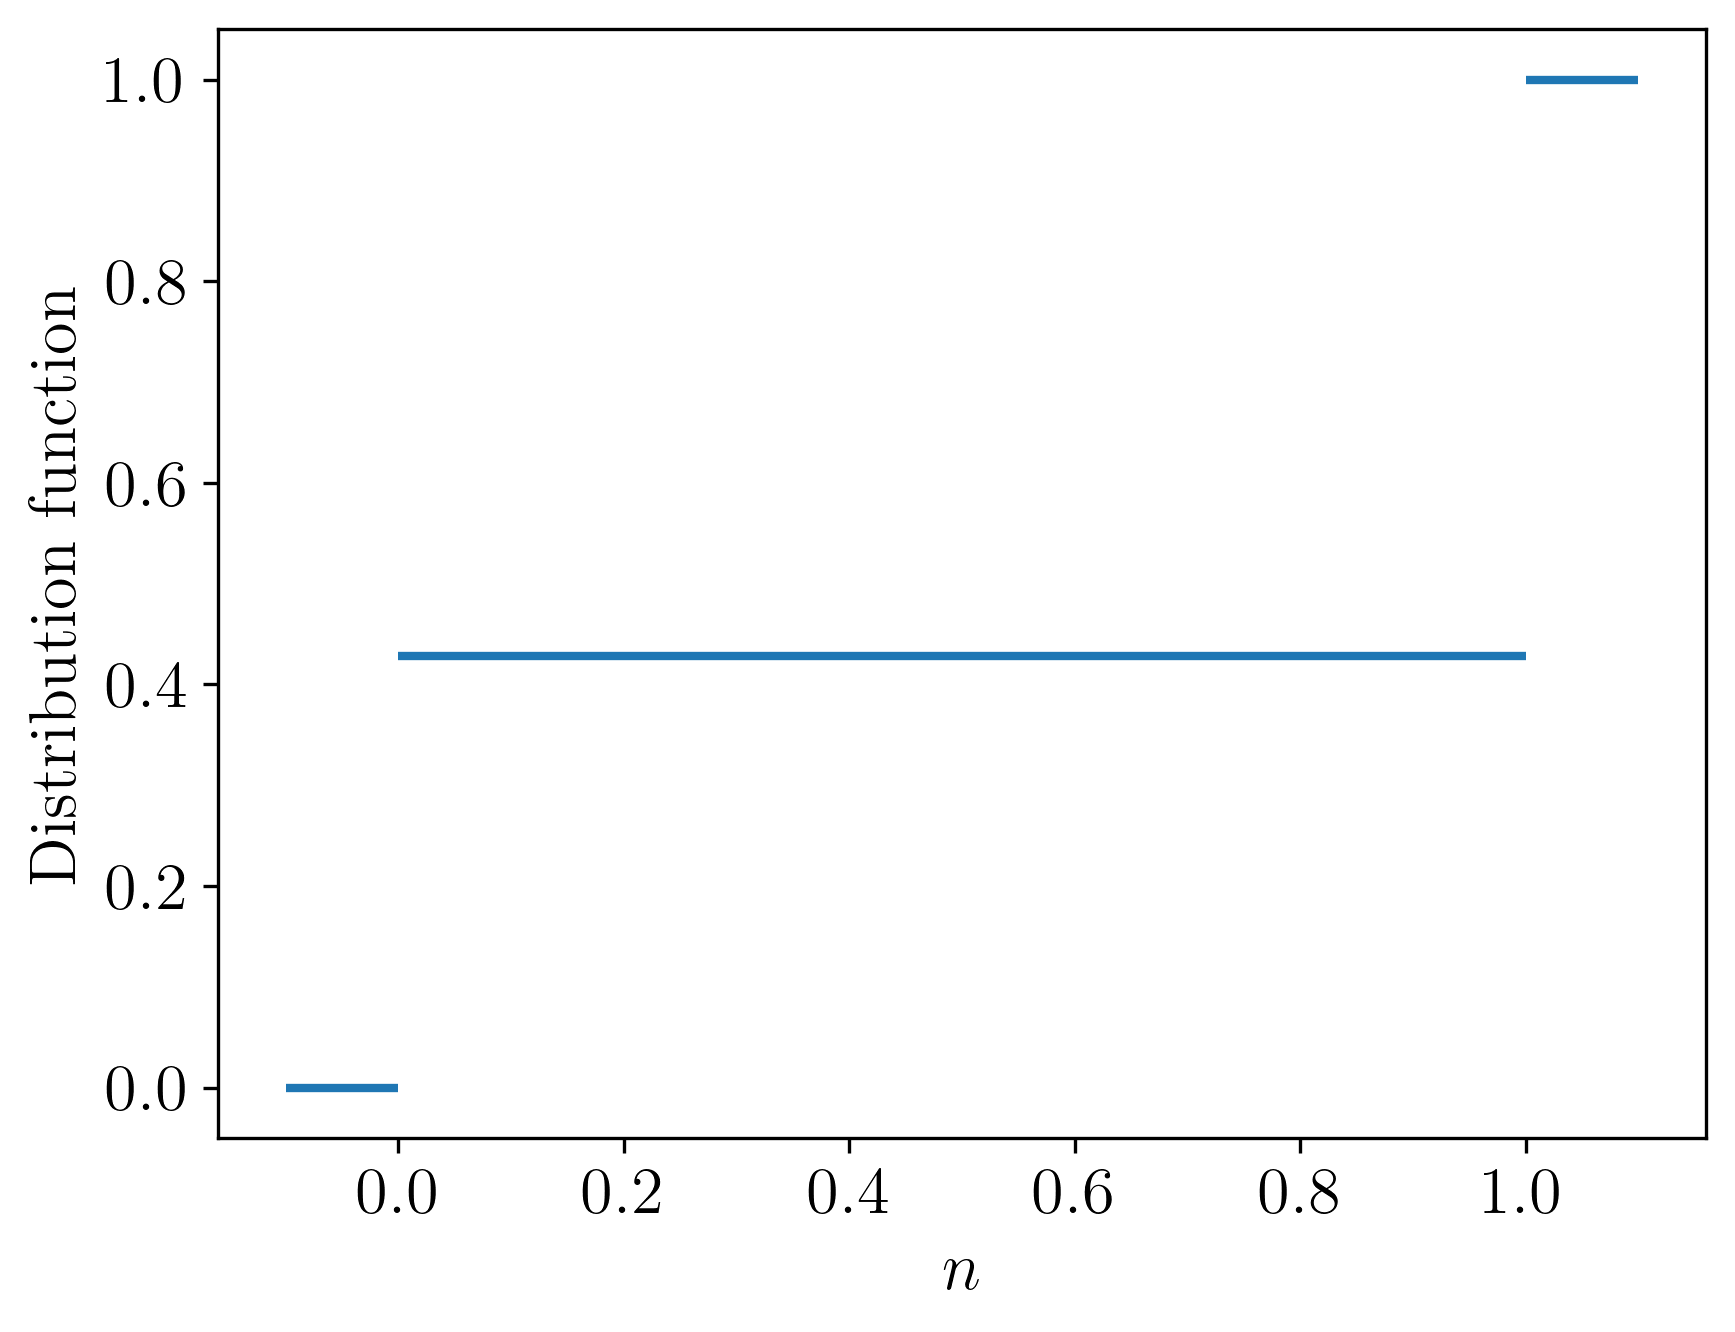
\includegraphics[width=.9\linewidth]{./Section/Grundlegende Begriffe/Verteilungsfunktion Bernoulli.png}
\vspace*{-.3\baselineskip}
\caption{\centering Verteilungsfunktion einer $\Ber(4/7)$-Verteilung}
\vspace*{-.3\baselineskip}
\end{center}
\end{figure}
\end{minipage}
\begin{minipage}{0.5\linewidth}
\begin{figure}[H]
\begin{center}
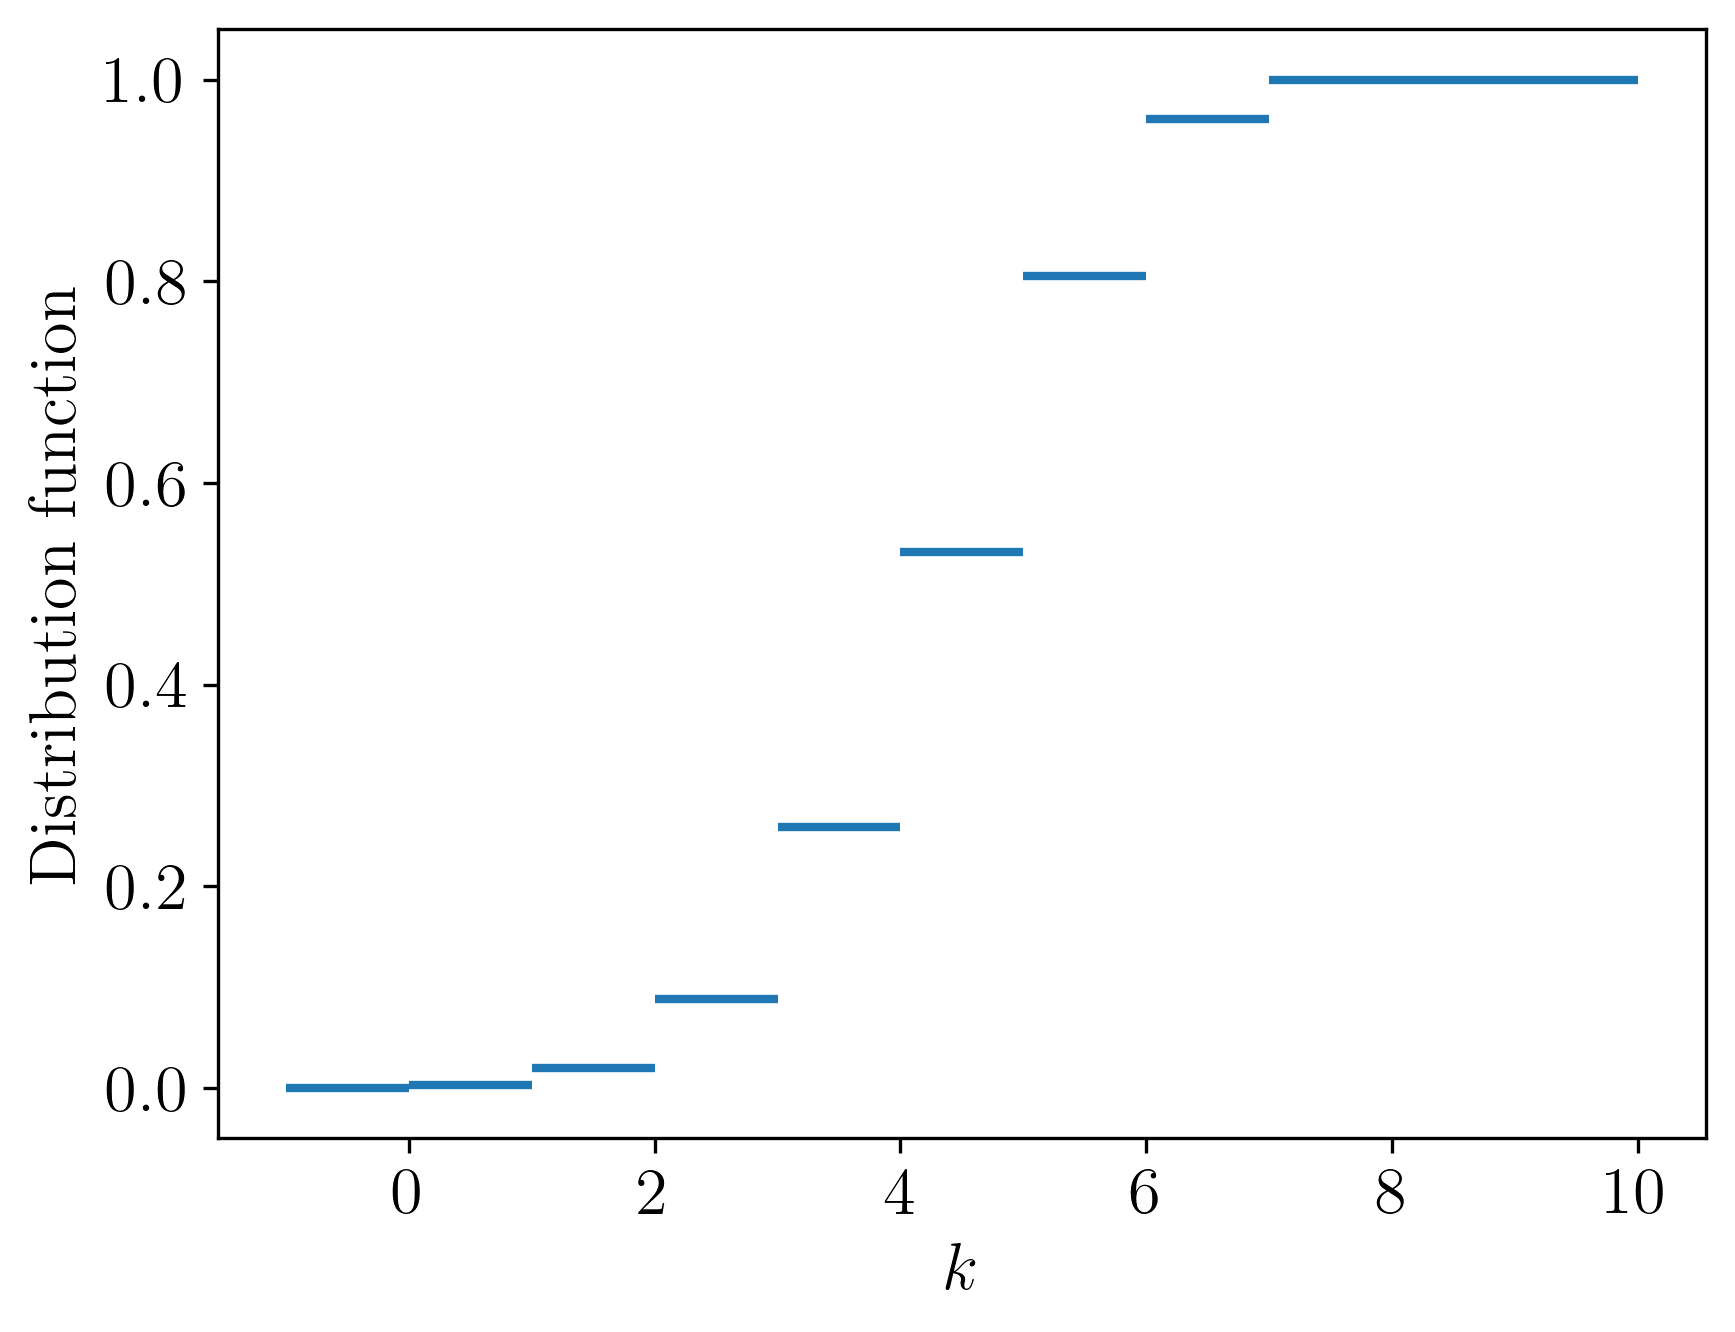
\includegraphics[width=.9\linewidth]{./Section/Grundlegende Begriffe/Verteilungsfunktion Binomial.png}
\vspace*{-.3\baselineskip}
\caption{\centering Verteilungsfunktion einer $\Bin(8, 2/3)$-Verteilung}
\vspace*{-.3\baselineskip}
\end{center}
\end{figure}
\end{minipage}
\vspace*{-\baselineskip}

\begin{minipage}{0.5\linewidth}
\begin{figure}[H]
\begin{center}
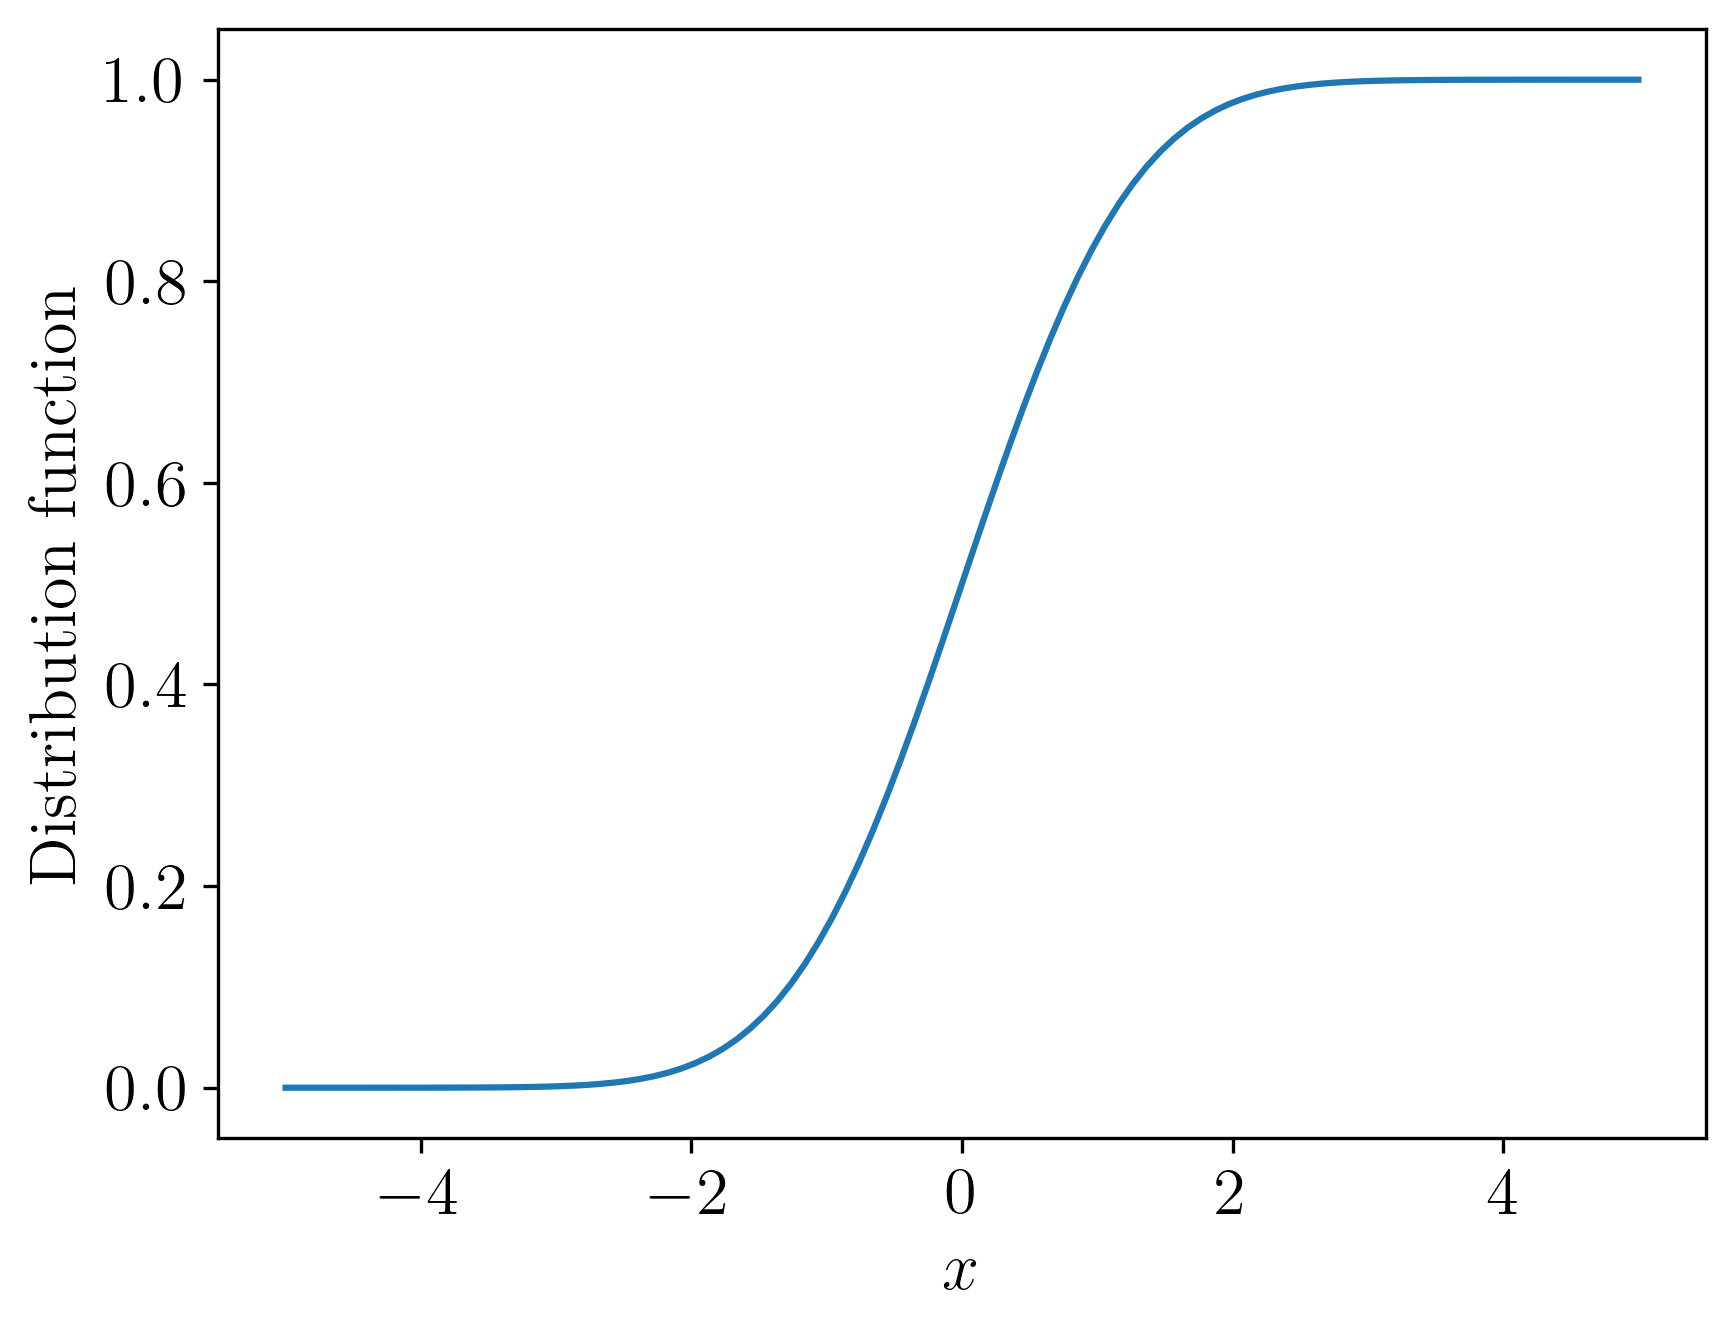
\includegraphics[width=.9\linewidth]{./Section/Grundlegende Begriffe/Verteilungsfunktion Normal.png}
\vspace*{-.3\baselineskip}
\caption{\centering Verteilungsfunktion einer $\Nor(0, 1)$-Verteilung}
\vspace*{-.3\baselineskip}
\end{center}
\end{figure}
\end{minipage}
\begin{minipage}{0.5\linewidth}
\begin{figure}[H]
\begin{center}
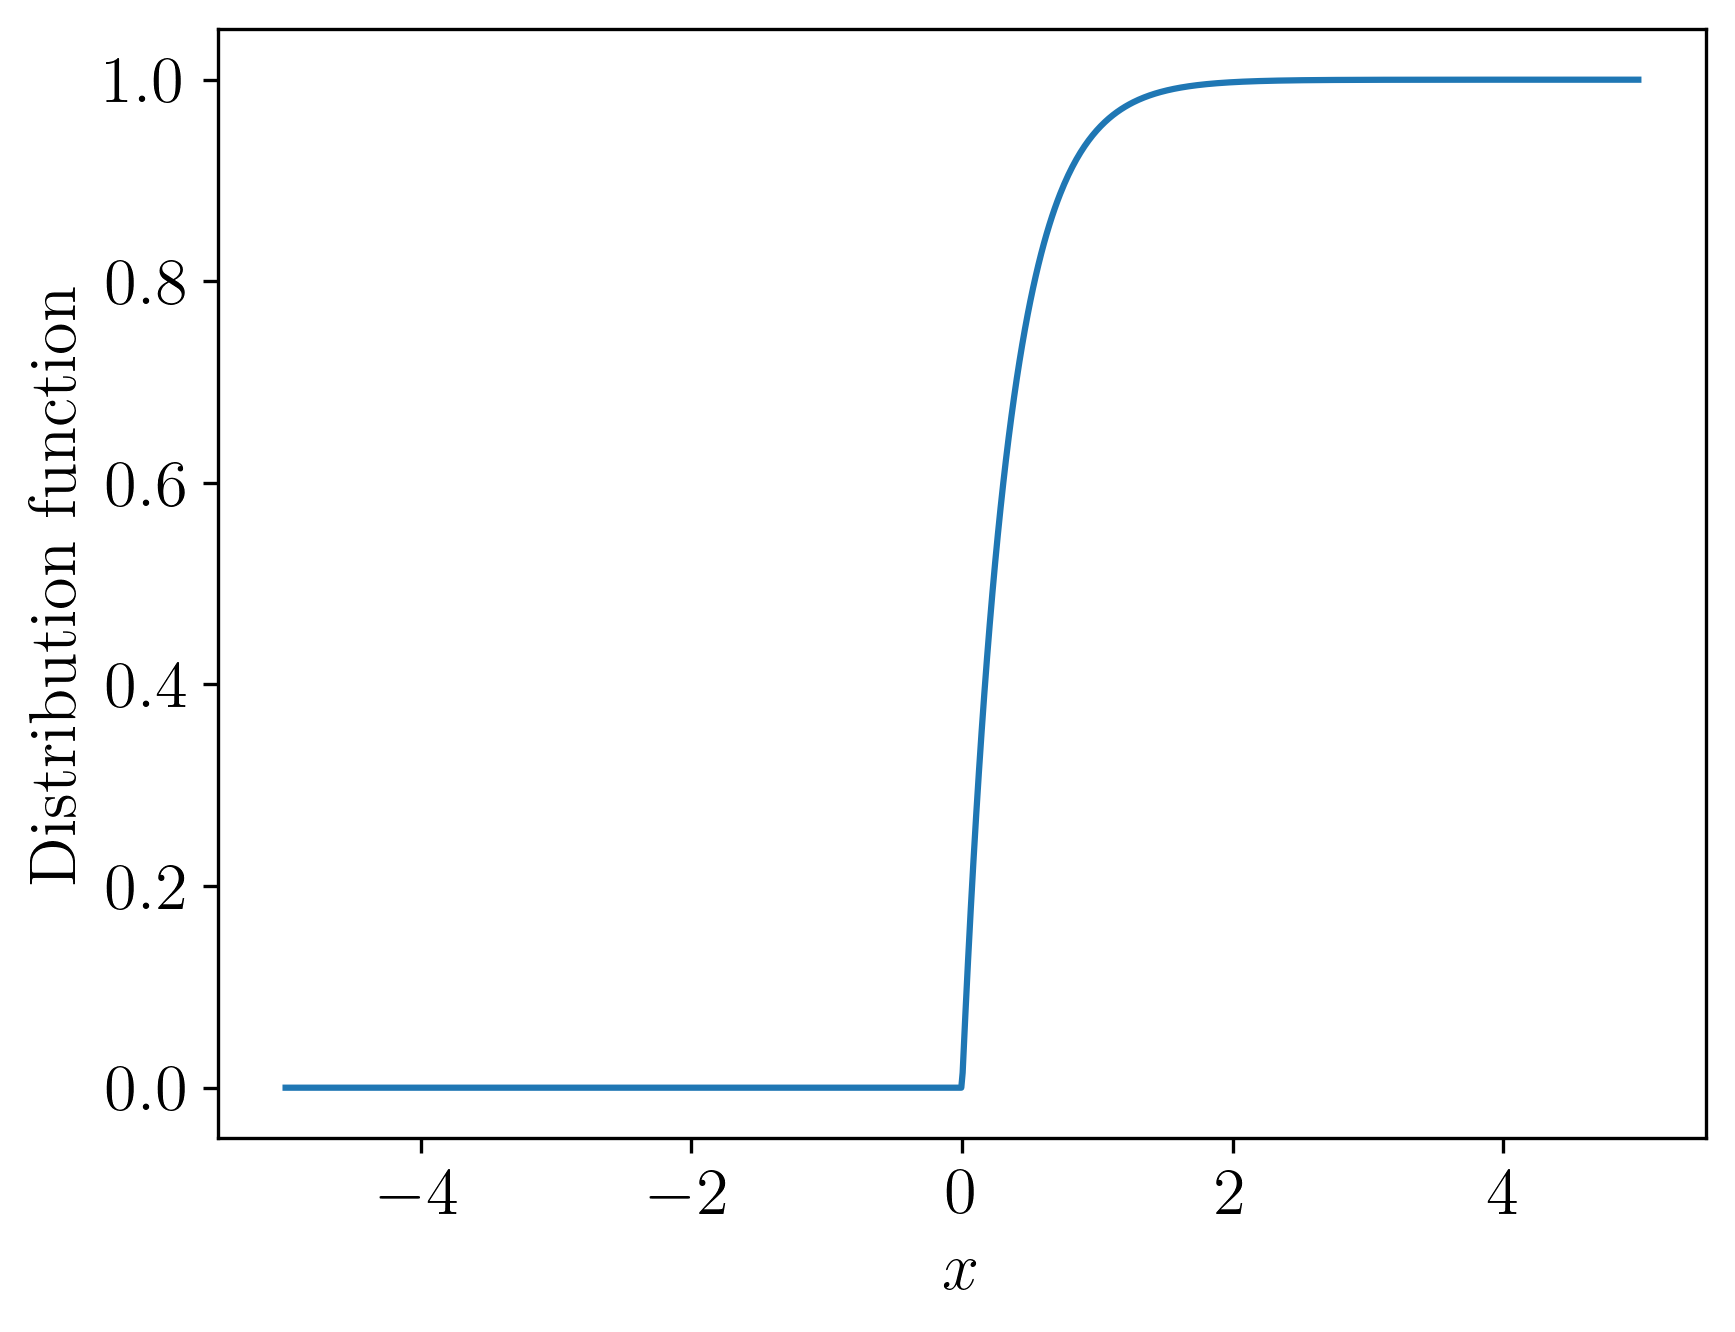
\includegraphics[width=.9\linewidth]{./Section/Grundlegende Begriffe/Verteilungsfunktion Exponential.png}
\vspace*{-.3\baselineskip}
\caption{\centering Verteilungsfunktion einer $\Exp(3)$-Verteilung}
\vspace*{-.3\baselineskip}
\end{center}
\end{figure}
\end{minipage}

Wir sehen bei allen Verteilungsfunktionen, dass sie nur Werte aus $[0, 1]$ annehmen und insbesondere die Grenzwerte $0$ und $1$ für $x \rightarrow -\infty$ und $x \rightarrow \infty$ haben. Außerdem sehen wir, dass Verteilungsfunktionen monoton wachsend sind. Bei der Bernoulli- und Binomialverteilung sehen wir deren stückweise stetige Natur. Die stetigen Verteilungen sind sogar stetig. Dies sind genau die Aussagen, die wir im \hyperlink{Satz:EigVertFun}{\blue{Satz über die Eigenschaften der Verteilungsfunktion}} gezeigt haben.
\end{Beispiel}
